\documentclass[a4paper,11pt]{article}
\pdfoutput=1 % if your are submitting a pdflatex (i.e. if you have
             % images in pdf, png or jpg format)
\usepackage{subcaption}

\usepackage{jinstpub} % for details on the use of the package, please
                     % see the JINST-author-manual
\usepackage{lineno}
\linenumbers
\def\myhyphen{{\hbox{-}}}
\usepackage{booktabs}
\usepackage{amsmath}
\title{\boldmath Measurement of cosmic-ray reconstruction efficiency in MicroBooNE using a small external cosmic-ray counter}

\collaboration{The MicroBooNE Collaboration}
%
% \author[g]{R.~Acciarri}
% \author[z]{C.~Adams}
% \author[h]{R.~An}
% \author[w]{J.~Asaadi}
% \author[a]{M.~Auger}
% \author[g]{L.~Bagby}
% \author[g]{B.~Baller}
% \author[q]{G.~Barr}
% \author[q]{M.~Bass}
% \author[x]{F.~Bay}
% \author[b]{M.~Bishai}
% \author[j]{A.~Blake}
% \author[i]{T.~Bolton}
% \author[m]{L.~Bugel}
% \author[f]{L.~Camilleri}
% \author[f]{D.~Caratelli}
% \author[g]{B.~Carls}
% \author[g]{R.~Castillo~Fernandez}
% \author[g]{F.~Cavanna}
% \author[b]{H.~Chen}
% \author[r]{E.~Church}
% \author[l,f]{D.~Cianci}
% \author[m]{G.~H.~Collin}
% \author[m]{J.~M.~Conrad}
% \author[u]{M.~Convery}
% \author[f]{J.~I.~Crespo-Anad\'{o}n}
% \author[q]{M.~Del~Tutto}
% \author[j]{D.~Devitt}
% \author[s]{S.~Dytman}
% \author[u]{B.~Eberly}
% \author[a]{A.~Ereditato}
% \author[c]{L.~Escudero Sanchez}
% \author[v]{J.~Esquivel}
% \author[z]{B.~T.~Fleming}
% \author[d]{W.~Foreman}
% \author[l]{A.~P.~Furmanski}
% \author[k]{G.~T.~Garvey}
% \author[f]{V.~Genty}
% \author[a]{D.~Goeldi}
% \author[i]{S.~Gollapinni}
% \author[s]{N.~Graf}
% \author[z]{E.~Gramellini}
% \author[g]{H.~Greenlee}
% \author[e]{R.~Grosso}
% \author[q]{R.~Guenette}
% \author[z]{A.~Hackenburg}
% \author[v]{P.~Hamilton}
% \author[m]{O.~Hen}
% \author[l]{J.~Hewes}
% \author[l]{C.~Hill}
% \author[d]{J.~Ho}
% \author[i]{G.~Horton-Smith}
% \author[g]{C.~James}
% \author[c]{J.~Jan~de~Vries}
% \author[y]{C.-M.~Jen}
% \author[s]{L.~Jiang}
% \author[e]{R.~A.~Johnson}
% \author[m]{B.~J.~P.~Jones}
% \author[b]{J.~Joshi}
% \author[g]{H.~Jostlein}
% \author[f]{D.~Kaleko}
% \author[l,f]{G.~Karagiorgi}
% \author[g]{W.~Ketchum}
% \author[b]{B.~Kirby}
% \author[g]{M.~Kirby}
% \author[g]{T.~Kobilarcik}
% \author[a]{I.~Kreslo}
% \author[q]{A.~Laube}
% \author[b]{Y.~Li}
% \author[j]{A.~Lister}
% \author[h]{B.~R.~Littlejohn}
% \author[g]{S.~Lockwitz}
% \author[a]{D.~Lorca}
% \author[k]{W.~C.~Louis}
% \author[a]{M.~Luethi}
% \author[g]{B.~Lundberg}
% \author[z]{X.~Luo}
% \author[g]{A.~Marchionni}
% \author[y]{C.~Mariani}
% \author[c]{J.~Marshall}
% \author[h]{D.~A.~Martinez~Caicedo}
% \author[i]{V.~Meddage}
% \author[o]{T.~Miceli}
% \author[k]{G.~B.~Mills}
% \author[m]{J.~Moon}
% \author[b]{M.~Mooney}
% \author[g]{C.~D.~Moore}
% \author[n]{J.~Mousseau}
% \author[l]{R.~Murrells}
% \author[s]{D.~Naples}
% \author[t]{P.~Nienaber}
% \author[j]{J.~Nowak}
% \author[g]{O.~Palamara}
% \author[s]{V.~Paolone}
% \author[o]{V.~Papavassiliou}
% \author[o]{S.F.~Pate}
% \author[g]{Z.~Pavlovic}
% \author[l]{D.~Porzio}
% \author[v]{G.~Pulliam}
% \author[b]{X.~Qian}
% \author[g]{J.~L.~Raaf}
% \author[i]{A.~Rafique}
% \author[u]{L.~Rochester}
% \author[a]{C.~Rudolf~von~Rohr}
% \author[z]{B.~Russell}
% \author[d]{D.~W.~Schmitz}
% \author[g]{A.~Schukraft}
% \author[f]{W.~Seligman}
% \author[f]{M.~H.~Shaevitz}
% \author[a]{J.~Sinclair}
% \author[g]{E.~L.~Snider}
% \author[v]{M.~Soderberg}
% \author[l]{S.~S{\"o}ldner-Rembold}
% \author[q,1]{S.~R.~Soleti\note{Corresponding author.}}
% \author[g]{P.~Spentzouris}
% \author[n]{J.~Spitz}
% \author[e]{J.~St.~John}
% \author[g]{T.~Strauss}
% \author[l]{A.~M.~Szelc}
% \author[p]{N.~Tagg}
% \author[f]{K.~Terao}
% \author[c]{M.~Thomson}
% \author[g]{M.~Toups}
% \author[u]{Y.-T.~Tsai}
% \author[z]{S.~Tufanli}
% \author[u]{T.~Usher}
% \author[k]{R.~G.~Van~de~Water}
% \author[b]{B.~Viren}
% \author[a]{M.~Weber}
% \author[c]{J.~Weston}
% \author[s]{D.~A.~Wickremasinghe}
% \author[g]{S.~Wolbers}
% \author[m]{T.~Wongjirad}
% \author[o]{K.~Woodruff}
% \author[g]{T.~Yang}
% \author[g]{G.~P.~Zeller}
% \author[d]{J.~Zennamo}
% \author[b]{C.~Zhang}
%
% % Institutions in alphabetical order
% \affiliation[a]{Universit{\"a}t Bern, Bern CH-3012, Switzerland}
% \affiliation[b]{Brookhaven National Laboratory (BNL), Upton, NY, 11973, USA}
% \affiliation[c]{University of Cambridge, Cambridge CB3 0HE, United Kingdom}
% \affiliation[d]{University of Chicago, Chicago, IL, 60637, USA}
% \affiliation[e]{University of Cincinnati, Cincinnati, OH, 45221, USA}
% \affiliation[f]{Columbia University, New York, NY, 10027, USA}
% \affiliation[g]{Fermi National Accelerator Laboratory (FNAL), Batavia, IL 60510, USA}
% \affiliation[h]{Illinois Institute of Technology (IIT), Chicago, IL 60616, USA}
% \affiliation[i]{Kansas State University (KSU), Manhattan, KS, 66506, USA}
% \affiliation[j]{Lancaster University, Lancaster LA1 4YW, United Kingdom}
% \affiliation[k]{Los Alamos National Laboratory (LANL), Los Alamos, NM, 87545, USA}
% \affiliation[l]{The University of Manchester, Manchester M13 9PL, United Kingdom}
% \affiliation[m]{Massachusetts Institute of Technology (MIT), Cambridge, MA, 02139, USA}
% \affiliation[n]{University of Michigan, Ann Arbor, MI, 48109, USA}
% \affiliation[o]{New Mexico State University (NMSU), Las Cruces, NM, 88003, USA}
% \affiliation[p]{Otterbein University, Westerville, OH, 43081, USA}
% \affiliation[q]{University of Oxford, Oxford OX1 3RH, United Kingdom}
% \affiliation[r]{Pacific Northwest National Laboratory (PNNL), Richland, WA, 99352, USA}
% \affiliation[s]{University of Pittsburgh, Pittsburgh, PA, 15260, USA}
% \affiliation[t]{Saint Mary's University of Minnesota, Winona, MN, 55987, USA}
% \affiliation[u]{SLAC National Accelerator Laboratory, Menlo Park, CA, 94025, USA}
% \affiliation[v]{Syracuse University, Syracuse, NY, 13244, USA}
% \affiliation[w]{University of Texas, Arlington, TX, 76019, USA}
% \affiliation[x]{TUBITAK Space Technologies Research Institute, METU Campus, TR-06800, Ankara, Turkey}
% \affiliation[y]{Center for Neutrino Physics, Virginia Tech, Blacksburg, VA, 24061, USA}
% \affiliation[z]{Yale University, New Haven, CT, 06520, USA}
%
%
% \emailAdd{stefano.soleti@physics.ox.ac.uk}




\abstract{The MicroBooNE detector is a Liquid Argon Time Projection Chamber designed for short-baseline neutrino physics, currently running at Fermilab. Due to its location near the surface, cosmic muons can be a source of backgrounds to several analyses and a good understanding of them is of fundamental importance for the experiment. This study presents a method of using an external muon counter system to determine the cosmic-ray reconstruction efficiency in MicroBooNE.
Data has been acquired with the external muon counter system placed in the three different positions, corresponding to cosmic rays intersecting different parts of the detector.
%The reconstruction of the tracks is performed using the multi-algorithm Pandora framework.
The data reconstruction efficiency is found to be $\epsilon_{\mathrm{data}}=97.1\pm0.1~(\mathrm{stat}) \pm 1.4~(\mathrm{sys})\%$, in good agreement with the Monte Carlo reconstruction efficiency $\epsilon_{\mathrm{MC}} = 97.3\pm0.1\%$.
This analysis represents a small-scale demonstration of the method that can be used with future data coming from the recently installed Cosmic Ray Tagger, which is able to tag $\sim80\%$ of the cosmic rays passing through the MicroBooNE detector.}

\keywords{Time projection chambers; Pattern recognition, cluster finding, calibration and fitting methods; Performance of High Energy Physics Detectors}


%\arxivnumber{1234.56789} % only if you have one



\begin{document}
\maketitle
\flushbottom

\section{Introduction}
\label{sec:intro}
MicroBooNE (Micro Booster Neutrino Experiment) is a Liquid Argon Time Projection Chamber (LArTPC) experiment located at the Fermi National Accelerator Laboratory (Fermilab) \cite{detector}. The main physics goals of the experiment are to investigate the excess of low-energy events, observed by the MiniBooNE experiment \cite{miniboone}, and to measure neutrino-argon cross sections. MicroBooNE also provides important research and development contributions in terms of detector technology and event reconstruction techniques for future LArTPC experiments, such as DUNE (Deep Underground Neutrino Experiment) \cite{dune}.

The MicroBooNE detector  consists of a rectangular time projection chamber (TPC) with dimensions of 256 cm $\times$ 233 cm $\times$ 1037 cm and is located 470 m away from the Booster Neutrino Beam (BNB) target. The x-direction of the TPC corresponds to the drift coordinate, the y-direction is the vertical direction, and the z-direction is the direction along the beam. The cylindrical cryostat contains a total of 170 ton of liquid argon, while the mass of liquid argon in the active volume, defined as the portion of the argon encompassed by the TPC, is 89 ton. Figure \ref{fig:coord} shows a graphical representation of the TPC in the MicroBooNE coordinate system.

\begin{figure}[htbp]
  \begin{center}
    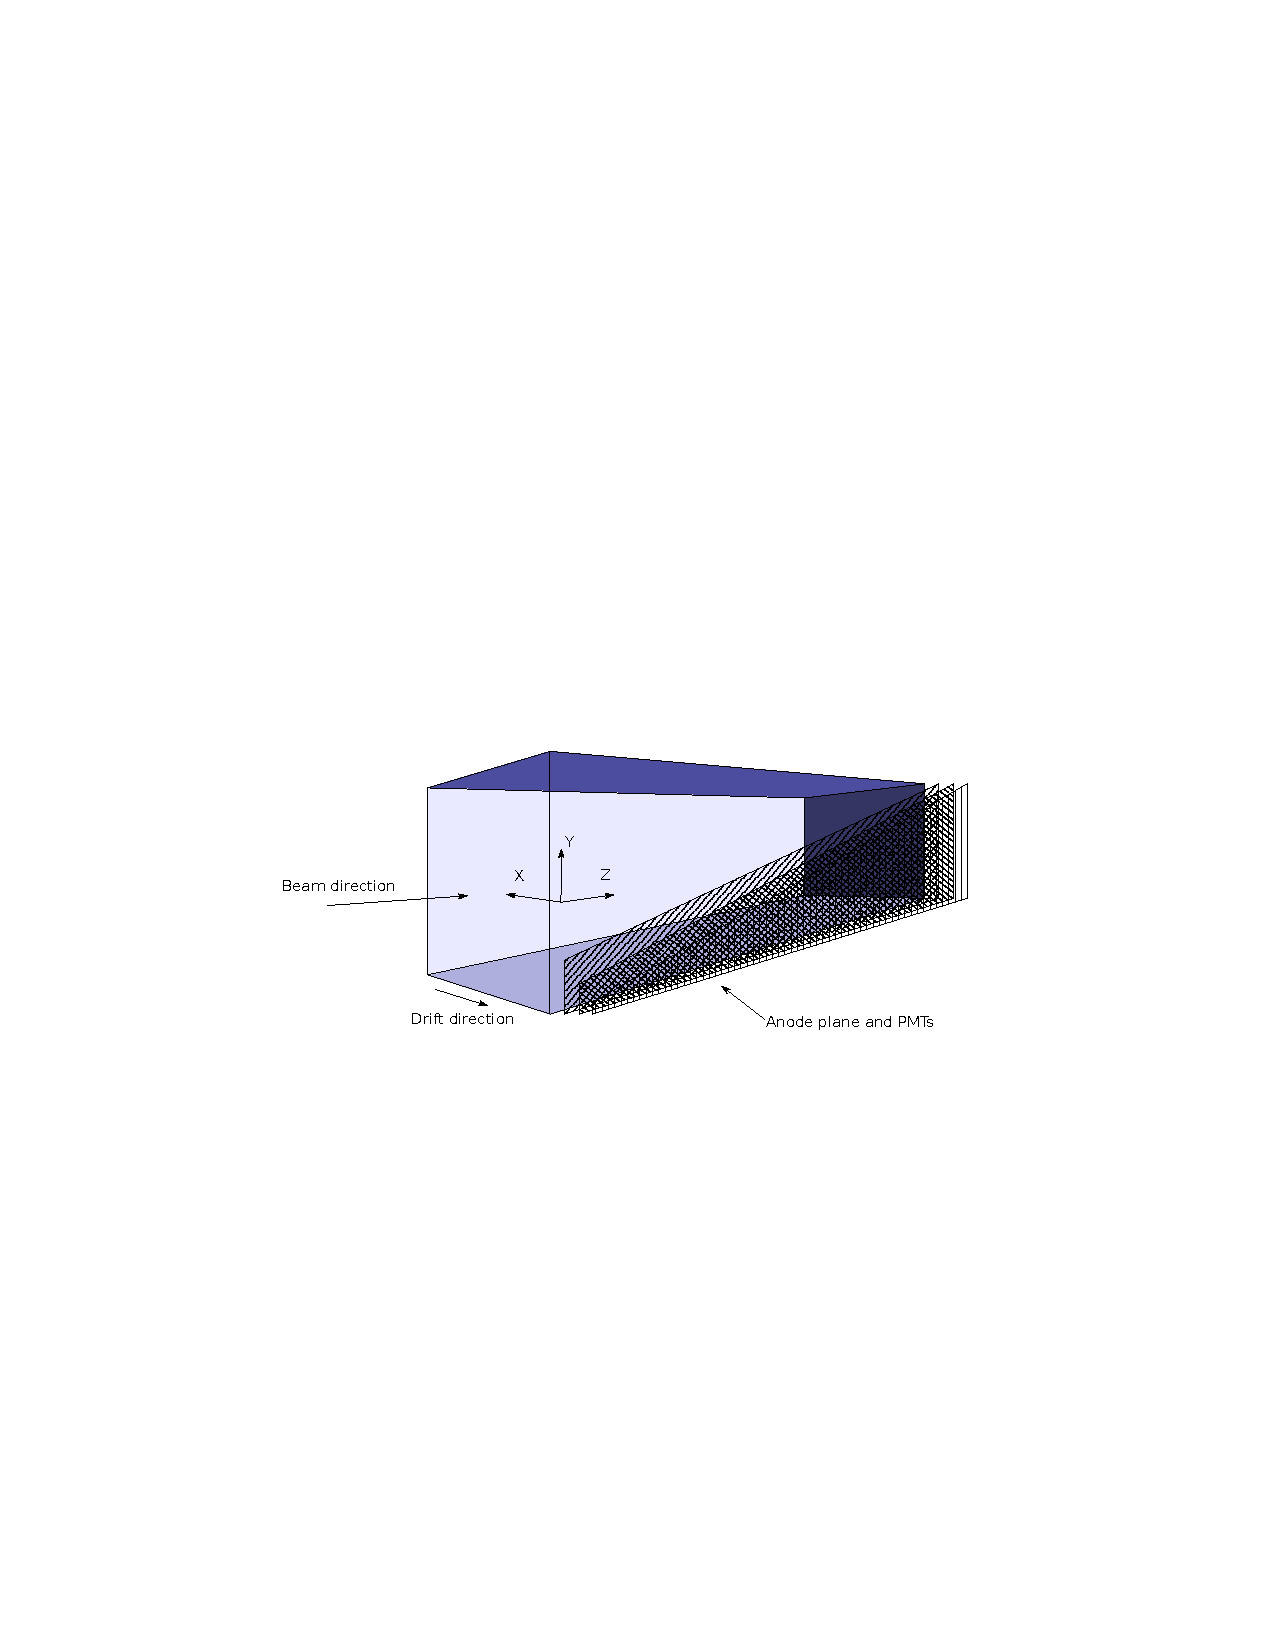
\includegraphics[width=0.8\linewidth]{figures/coord.pdf}

    \caption{The MicroBooNE coordinate system. The three wire planes, shown in the right front face, are vertical (collection plane) and at  $\pm60^{\circ}$ to the vertical (induction planes). The dimensions of the TPC are 256 cm $\times$ 233 cm $\times$ 1037 cm (x $\times$ y $\times$ z). The coordinate system is explained in detail in \cite{mcdata}. The figure is taken from \cite{mcdata}.} \label{fig:coord}
  \end{center}
\end{figure}

The TPC consists of an anode made of three wire planes with 3 mm spacing at angles of 0,  $+60^{\circ}$ and  $-60^{\circ}$ with respect to the vertical. The cathode, made of stainless steel sheets, operates at a voltage of -70 kV. In a neutrino interaction, a neutrino from the beam interacts with an argon nucleus and the secondary charged particles traverse the medium, losing energy and leaving an ionization trail. The resulting ionization electrons drift to the wire planes under an electric field of 273 V/cm. The distance between the cathode and anode is 2.56 m and an ionization electron takes about 2.2 ms to travel the full drift distance, called the drift time window. The passage of these electrons near the wire planes induces a signal used to create three distinct two-dimensional views (in terms of wire and time) of the event.

A set of 32 photomultipliers tubes (PMTs) is placed behind the anode plane to collect the argon scintillation light. Scintillation light provides timing information with few-nanosecond precision, that, combined to the wire signals, allows for full three-dimensional reconstruction of the event. More details about the MicroBooNE detector can be found in \cite{detector}.

The BNB is predominantly composed of muon neutrinos ($\nu_{\mu}$) with a peak neutrino energy of about 0.7 GeV, which can undergo charge-current ($\nu_{\mu}$CC) interactions in the TPC and produce muons. Due to the shallow depth of the detector location (around 6 meters below surface level), the abundant flux of cosmic muons can be a source of background to neutrino events and an optimal reconstruction of the cosmic rays in the TPC is crucial. The muon cosmic-ray flux in the MicroBooNE detector is estimated to be at the rate of 5.5 kHz, which corresponds to approximately 12 muons per TPC drift time window (2.2 ms) \cite{cosmic}.

This paper describes a measurement of the reconstruction efficiencies using a dataset of cosmic rays triggered by an external Muon Counter System (MuCS) and passing through the MicroBooNE TPC. The goals are to provide data and Monte Carlo reconstruction efficiencies that can be used to evaluate reconstruction performance and to show that an external cosmic-ray counter can be used to measure the data reconstruction efficiency in MicroBooNE.

The description of the MuCS is given in section \ref{sec:proc}. A discussion of the data processing and analysis, as well as the Monte Carlo simulations is presented in section \ref{sec:merging}. The details of the reconstruction efficiency measurements and comparison and of the evaluation of the systematic uncertainties are given in section \ref{sec:reco}.

%The data reconstruction efficiency is calculated comparing the number of events triggered by the MuCS and the number of events with a MuCS-compatible reconstructed track in the TPC.
%The Monte Carlo reconstruction efficiency is measured by comparing the number of generated cosmic rays with the number of reconstructed tracks, using simulated cosmic rays hitting the entire TPC.

%The reconstruction efficiency is expressed as a function of the cosmic-ray starting angle (given by the spherical angles $\theta$ and $\phi$ relative to the beam direction $+z$) and of the expected length $L$ of its path in the TPC. More details on the Monte Carlo generation can be found in section \ref{sec:merging}.%, assuming it is a minimum-ionizing particle (MIP).

%Using the Pandora pattern-recognition software framework \cite{pandora}, the overall reconstruction efficiency is $97.1\pm0.1\thinspace(\mathrm{stat}) \pm 1.4\thinspace(\mathrm{sys})\thinspace\%$ for data and $97.3\pm0.1\thinspace\%$ for Monte Carlo.

In the future, the method described in this paper can be adapted to use the data coming form the Cosmic Ray Tagger (CRT) system \cite{crt}. The CRT system has been installed in the summer of 2016 and it is able to tag around 80\% of the cosmic rays hitting the MicroBooNE LArTPC. The larger data sample provided by the CRT will offer a larger coverage of the detector regions  and measure efficiency-corrected quantities for the whole detector, such as the cosmic-ray flux in the TPC, will be measured.


\section{The Muon Counter System}\label{sec:proc}
The Muon Counter System, described in detail in \cite{mucs}, consists of two sets of planar modules placed into two separate, light-tight boxes. The upper and lower boxes are placed 2.75 m and 2.03 m above the TPC, respectively. Each planar module is made up of two sets of 24 scintillator strips, 4 cm wide, arranged into bi-layers oriented perpendicular to each other, as shown in figure \ref{fig:boxes}. Each strip contains a wavelength shifting optical fiber, connected to a Multi-Anode PMT. The Multi-Anode PMTs are read out by a dedicated DAQ system, which records the hit patterns of the scintillator stripes.
The MuCS is designed to provide a trigger on through-going muons that intersect all four bi-layers of scintillator strips. The MuCS trigger is propagated to the MicroBooNE trigger board and provides the starting time ($t_0$) of a track in the TPC associated with the MuCS.
%The MuCS DAQ that reads out the Multi-Anode PMTs is separated from the DAQ system that reads out the TPC and PMT systems of the main detector. It records the hit patterns of the scintillator stripes, while the main DAQ stores the TPC and PMT signals during the readout time window.

As illustrated in Figure \ref{fig:boxes}, a signal in one strip corresponds to a MuCS hit and, combining the MuCS hits in each bi-layer, it is possible to obtain two sets of position coordinates of the crossing points of the cosmic rays (the $z$ and $x$ coordinates in the MicroBooNE TPC reference frame shown in figure \ref{fig:coord}). The height of the modules (corresponding to the $y$ coordinate for the MicroBooNE TPC reference frame), known to a precision of 0.5 cm, allows to extrapolate a three-dimensional trajectory of the cosmic ray from the MuCS down to the TPC, which is defined as a \emph{MuCS-extrapolated track}.
\begin{figure}[htbp]
  \begin{center}
    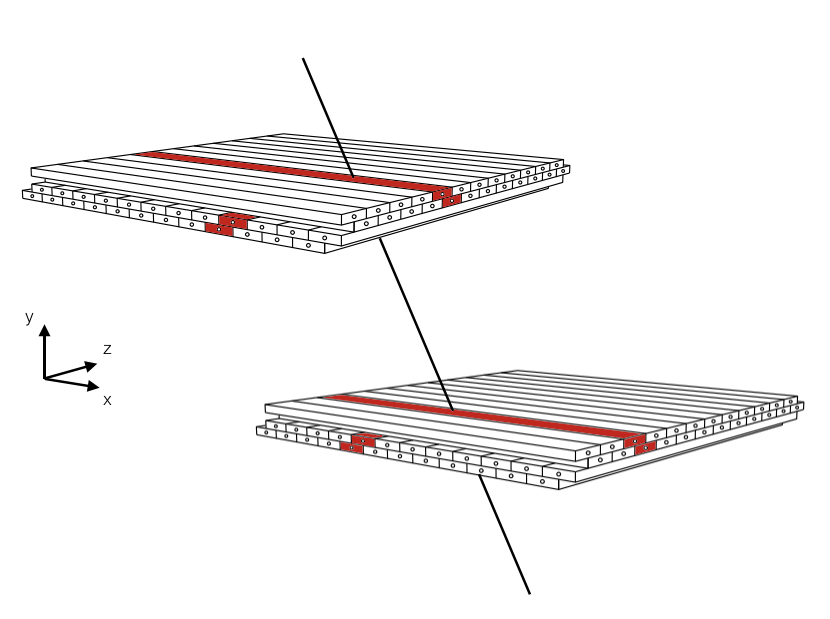
\includegraphics[width=0.7\linewidth]{figures/boxes.png}
    \caption{A cosmic ray passing through the MuCS boxes hits the scintillator strips, producing a signal that is defined as a MuCS hit. From the height of the panels and the position of the hit strips (highlighted in red) it is possible to extrapolate the trajectory of the cosmic ray down to the TPC located below.} \label{fig:boxes}
  \end{center}
\end{figure}

The starting angle of the cosmic ray trajectory, in spherical coordinates, is defined by:
\begin{align}\label{eq:angles}
  \theta = \mathrm{acos}\left(\frac{z_{\mathrm{top}}-z_{\mathrm{bottom}}}{r}\right), \quad
  \phi = \mathrm{atan}\left(\frac{y_{\mathrm{top}}-y_{\mathrm{bottom}}}{x_{\mathrm{top}}-x_{\mathrm{bottom}}}\right),
\end{align}
where $r = \sqrt{(x_{\mathrm{top}}-x_{\mathrm{bottom}})^2+(y_{\mathrm{top}}-y_{\mathrm{bottom}})^2+(z_{\mathrm{top}}-z_{\mathrm{bottom}})^2}$ and the top (bottom) coordinates are given by the hit positions in the top (bottom) MuCS box.


This analysis has been performed on three datasets, acquired with different geometrical configurations. The three configurations correspond to a setup with the two boxes placed at the upstream end, at the center and at the downstream end of MicroBooNE, keeping the boxes spacing and alignment identical.
A three-dimensional schematic of the three MuCS setups is shown in figure \ref{fig:mucs}.

\begin{figure}[htbp]
  \begin{subfigure}{0.30\textwidth}
    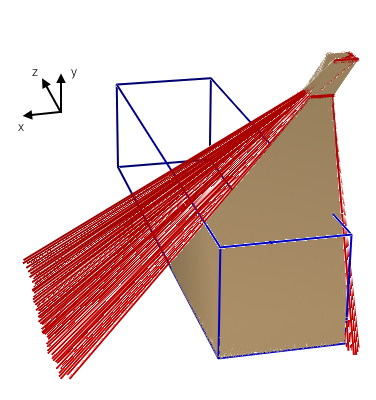
\includegraphics[width=\linewidth]{figures/upstream.png}
    \caption{Upstream} \label{fig:upstream}
  \end{subfigure}
  \begin{subfigure}{0.30\textwidth}
    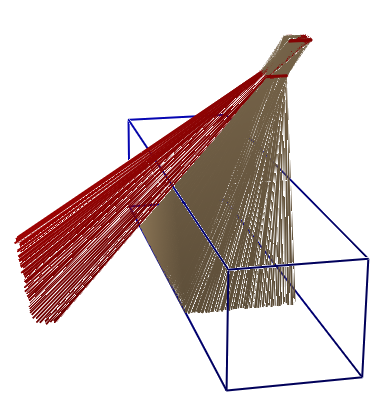
\includegraphics[width=\linewidth]{figures/center.png}
    \caption{Center} \label{fig:centre}
  \end{subfigure}
  \begin{subfigure}{0.30\textwidth}
    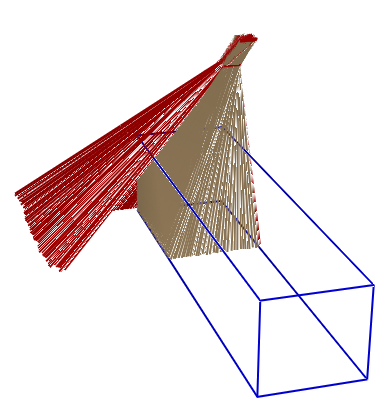
\includegraphics[width=\linewidth]{figures/downstream.png}
    \caption{Downstream} \label{fig:downstream}
  \end{subfigure}

  \caption{Illustration of the three MuCS configurations with a Monte Carlo simulation of the possible MuCS trajectories. Brown tracks correspond to cosmic rays hitting both MuCS boxes and the TPC, while red tracks go through only the MuCS and miss the TPC.} \label{fig:mucs}
\end{figure}


\section{MuCS data processing and Monte Carlo generation}\label{sec:merging}

\subsection{Data sample processing}\label{sec:data_proc}
The MuCS triggers at a rate of nearly 3 Hz. Given a MuCS DAQ integration window of 100 ns, the accidental coincidental rate of having more than one cosmic ray in the same integration window has estimated to be less then 0.01\% and it is considered negligible for this study. A software filter removes the events with more than 4 hit strips per bi-layer from the data sample, further reducing this accidental rate.
The probability that, during a same drift time window of 2.2 ms, a second cosmic ray crosses the MuCS and hit the TPC is, given a trigger rate of 3 Hz, 0.01\% and it is also considered negligible for this study. Therefore, it is assumed for this study that only one cosmic ray per drift time window is going through the MuCS and the TPC.

The data follows a processing path that merges the MuCS hit patterns and extrapolated trajectory information with the TPC and PMT data streams to form a MuCS-merged dataset. %A flowchart of the procedure is shown in figure \ref{fig:scheme}.

% \begin{figure}[htbp]
%   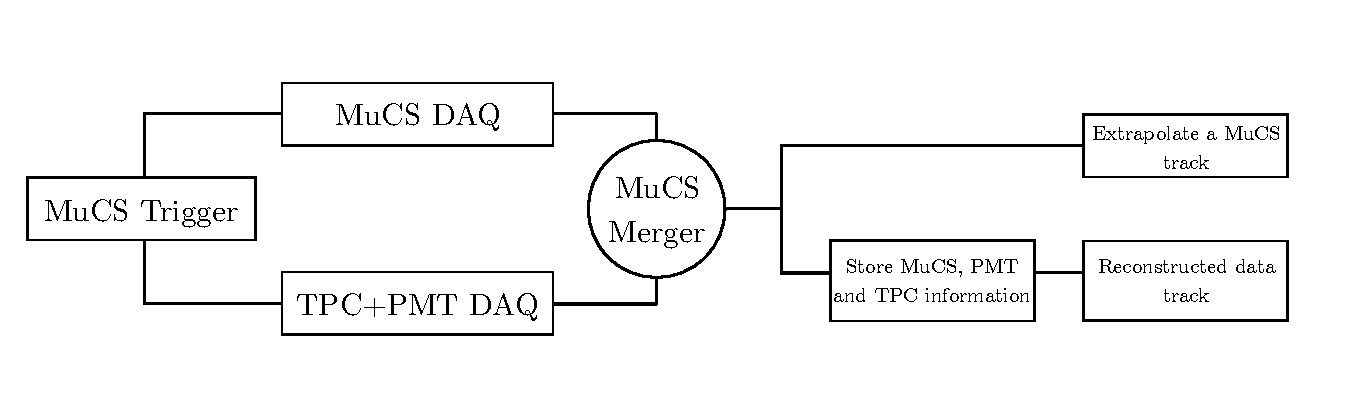
\includegraphics[width=\linewidth]{figures/scheme.pdf}
%   \caption{Flowchart showing the procedure used to generate the dataset used in this analysis. We end up with two data products: one with extrapolated coordinates obtained using MuCS-only data and one with reconstructed TPC tracks and PMT flashes, if present.} \label{fig:scheme}
% \end{figure}

The hits in the MuCS are used to obtain a point for each box and extrapolate a track through the TPC (MuCS-extrapolated track) as described in section \ref{sec:proc}. The ionized electrons generate a signal in the TPC wires to form the TPC hits, that are then fed to the MicroBooNE reconstruction chain and used by the track reconstruction algorithms provided by the Pandora framework \cite{pandora} to form the TPC reconstructed tracks.

The first intersection point between the MuCS-extrapolated track and the TPC is defined as $(x_{\mathrm{MuCS}}$, $y_{\mathrm{MuCS}}$, $z_{\mathrm{MuCS}})$. However, because of the multiple Coulomb scattering in the space between the MuCS boxes and the TPC, the starting point of the reconstructed track corresponding to the MuCS-triggering cosmic ray does not coincide exactly with the extrapolated intersection point $(x_{\mathrm{MuCS}}$, $y_{\mathrm{MuCS}}$, $z_{\mathrm{MuCS}})$.

The TPC reconstructed track with the closest starting point to the MuCS-extrapolated track intersection point is stored in the dataset and is defined as a \emph{MuCS-tagged track}.

The distance $d$ between the extrapolated intersection point and the starting point of the MuCS-tagged track is defined as:
\begin{equation}\label{eq:d}
d = \sqrt{(x_{\mathrm{MuCS}}-x_{\mathrm{reco}})^2+(y_{\mathrm{MuCS}}-y_{\mathrm{reco}})^2+(z_{\mathrm{MuCS}}-z_{\mathrm{reco}})^2},
\end{equation}
where $(x_{\mathrm{reco}},y_{\mathrm{reco}},z_{\mathrm{reco}})$ is the starting point of the MuCS-tagged track.

 %We know that the space charge effect can displace the start and end points of the reconstructed tracks by a sensible amount (around 15 cm for points near the cathode), so we correct this displacement with the procedure described in \cite{sce}.
%A PMT flash is associated with the MuCS signal if it falls within a well-known window with respect to the MuCS trigger.
Figure \ref{fig:evd} shows a diagram with the MuCS-extrapolated track (black line), the MuCS-tagged track (green line) and the other reconstructed cosmic-ray tracks in the TPC in the same readout window (grey lines). The distance $d$ between the first intersection point and the starting point of the MuCS-tagged track is shown by the red double-headed arrow.

\begin{figure}[htbp]
  \begin{center}
  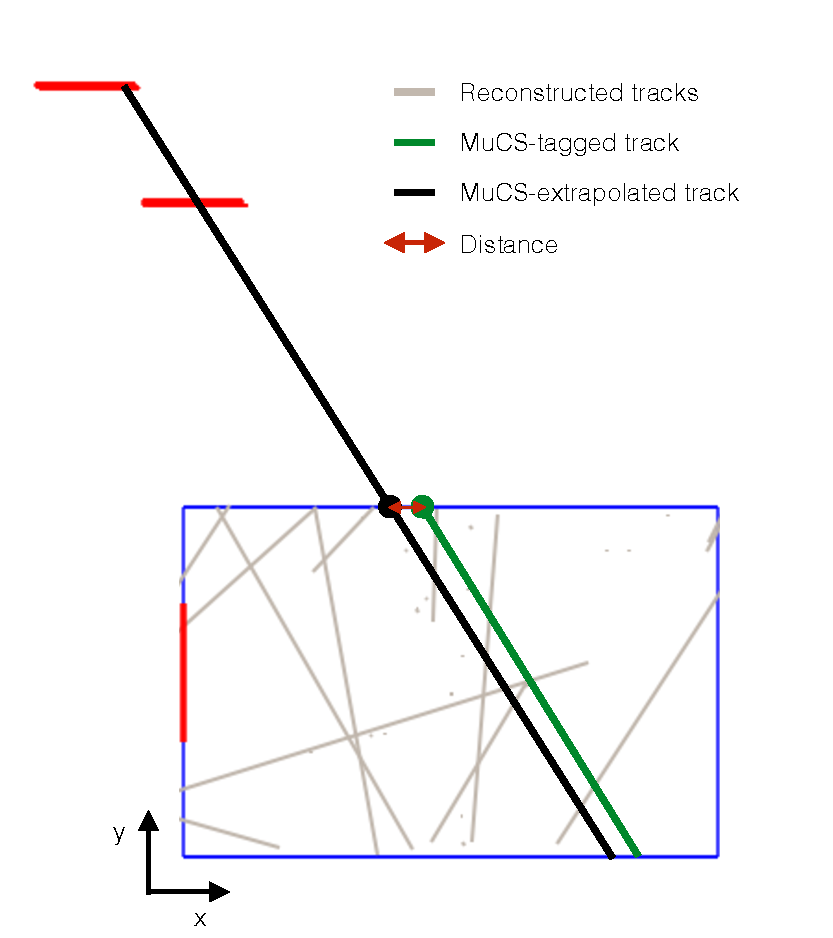
\includegraphics[width=0.50\linewidth]{figures/evd.pdf}
  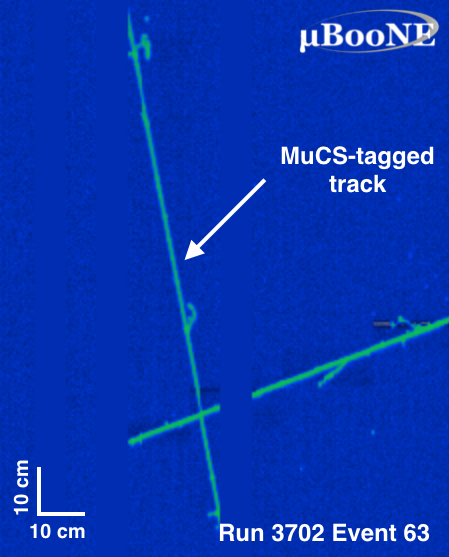
\includegraphics[width=0.40\linewidth]{figures/evd_display.png}

  \caption{Left: bi-dimensional view of a MuCS event in the MicroBooNE event display schematic. The black line shows the MuCS-extrapolated track, while the green line corresponds to the MuCS-tagged track. The black and green dots correspond to the $(x_{\mathrm{MuCS}},y_{\mathrm{MuCS}},z_{\mathrm{MuCS}})$ and $(x_{\mathrm{reco}},y_{\mathrm{reco}},z_{\mathrm{reco}})$ coordinates, respectively. Right: example of a MicroBooNE event display for the collection plane, showing a MuCS-tagged track in a real data event.} \label{fig:evd}
\end{center}
\end{figure}

The data product will then include two different sets of information:
\begin{itemize}
  \item MuCS-extrapolated information: a line crossing the entire TPC is extrapolated from the two points given by the MuCS (one for each box). From this extrapolated line it is possible to obtain: (1) the two extrapolated starting angles $\theta$ and $\phi$ of the MuCS, defined in eq. \eqref{eq:angles}, (2) the extrapolated start point $(x_{\mathrm{MuCS}},y_{\mathrm{MuCS}},z_{\mathrm{MuCS}})$ described above, and (3) the extrapolated end point, corresponding to the second intersection between the MuCS-extrapolated track and the TPC, where the track exits. The extrapolated track length $L$ is calculated measuring the difference between the extrapolated start point and the extrapolated end point.
  \item Reconstructed TPC data information: for each MuCS-triggered event, the identified reconstructed starting point $(x_{\mathrm{reco}},y_{\mathrm{reco}},z_{\mathrm{reco}})$ of the MuCS-tagged track is stored.
\end{itemize}

\subsection{Monte Carlo sample generation}\label{sec:mcgen}

The Monte Carlo sample used for this work consists of a simulation of cosmic ray events in the MicroBooNE TPC, as described in \cite{cosmic}. The cosmic rays are produced using the CORSIKA \cite{corsika} simulation software. Then, the generated muons are propagated with GEANT4 \cite{geant} and passed through the detector simulation stage. The detector simulation reproduces detector response as precisely as possible, reflecting the current state of the detector. Some regions of the TPC, for example, contain noisy or unresponsive wires whose position is known and can make the track reconstruction more difficult. Their effect is fully simulated and their impact is discussed in detail in section \ref{sec:wires}.

Other known effects, such as the space charge effect, are not currently modeled in the simulation. The space charge effect is created by the build-up of slow-moving positive ions in a detector due to ionization from cosmic rays, leading to a small distortion of the electric field in the detector. This effect leads to a displacement in the reconstructed position of signal ionization electrons in LArTPCs, This effect is corrected in the data with the procedure described in \cite{sce}, which still allows direct comparison with the current Monte Carlo simulation.

The output of the detector simulation stage is fed to the reconstruction chain. A successfully reconstructed track will be associated to the generated cosmic ray.

The direction of the simulated cosmic ray is calculated using its starting momentum, given by GEANT4. The starting angles $\theta$ and $\phi$ are defined in this case as:

\begin{align}\label{eq:angles}
  \theta = \mathrm{acos}\left(\frac{p_{z}}{p}\right), \quad
  \phi = \mathrm{atan}\left(\frac{p_{y}}{p_{x}}\right),
\end{align}
where $p_{x}$, $p_{y}$, $p_{z}$ are the $x$, $y$, $z$ components of the cosmic-ray momentum of magnitude $p$.
The extrapolated track length $L$ is calculated extrapolating a line through the TPC and measuring the distance between the extrapolated start point and the extrapolated end point in the TPC.

This Monte Carlo simulation provides cosmic rays entering the TPC from all possible directions, while the cosmic rays triggering the MuCS can have only certain $\theta$, $\phi$ starting angles due to geometrical constraints of the system. Thus, cosmic rays in the Monte Carlo dataset are selected to match the ($\theta$, $\phi$) parameter space covered by the MuCS data.

%Our aim is to show that the reconstruction efficiency of simulated cosmic rays, generated all over the TPC, can be successfully compared to the data reconstruction efficiency, obtained placing the MuCS in three different places.

\section{Reconstruction efficiencies}\label{sec:reco}

The MuCS reconstruction efficiency $\epsilon$ is defined as the ratio between the number of events with a reconstructed MuCS cosmic ray and the number of MuCS-triggered events:
\begin{equation}\label{eq:eff}
  \epsilon = \frac{\mathrm{N.~of~reco.~MuCS~cosmic\myhyphen ray~events}}{\mathrm{N.~of~MuCS~triggered~events}}.
\end{equation}
In a data sample it is not possible to identify with certainty a MuCS cosmic ray and the MuCS-tagged track is defined as the reconstructed track with the closest starting point $(x_{\mathrm{reco}},y_{\mathrm{reco}},z_{\mathrm{reco}})$ to the extrapolated MuCS starting point $(x_{\mathrm{MuCS}},y_{\mathrm{MuCS}},z_{\mathrm{MuCS}})$, as shown in figure \ref{fig:evd}. Since some cosmic rays can trigger the MuCS without hitting the TPC (see red tracks in figure \ref{fig:mucs}), eq. \eqref{eq:eff} includes only the events with an extrapolated length in the TPC $L > 20$ cm, to ensure that the reconstruction efficiency is not being artificially lowered by including cosmic rays that missed the TPC or crossed it only for a very small path.

For every MuCS-triggered event there are on average 12 reconstructed tracks in the TPC. Therefore, events where the MuCS-triggered cosmic ray is not reconstructed are always associated to one other reconstructed cosmic ray, so it is necessary to enforce a maximum distance $d_{\mathrm{max}}$ between the two points, $(x_{\mathrm{reco}},y_{\mathrm{reco}},z_{\mathrm{reco}})$ and $(x_{\mathrm{MuCS}},y_{\mathrm{MuCS}},z_{\mathrm{MuCS}})$ to reduce misassociations. The number of events with a MuCS-tagged track will then depend on $d_{\mathrm{max}}$.

In order to study the dependence of the number of MuCS-tagged tracks on $d_{\mathrm{max}}$, a dedicated Monte Carlo simulation of a MuCS run is performed and defined as \emph{MuCS Monte Carlo}. Each event of this simulation has one cosmic ray passing through the MuCS boxes and several other cosmic rays hitting the TPC during the same time window.

In the MuCS Monte Carlo the truth information allows to verify if the MuCS-tagged cosmic ray is a real MuCS cosmic ray or if it is one unassociated reconstructed cosmic ray, which happens to be mis-identified due to the extrapolated starting point distance being closer than $d_{\mathrm{max}}$ because of multiple Coulomb scattering.
The distance $d$ is defined in this case as:
\begin{equation}\label{eq:d_mc}
d = \sqrt{(x_{\mathrm{sim}}-x_{\mathrm{reco}})^2+(y_{\mathrm{sim}}-y_{\mathrm{reco}})^2+(z_{\mathrm{sim}}-z_{\mathrm{reco}})^2},
\end{equation}
where $(x_{\mathrm{sim}},y_{\mathrm{sim}},z_{\mathrm{sim}})$ and $(x_{\mathrm{reco}},y_{\mathrm{reco}},z_{\mathrm{reco}})$ are the coordinates of the intersection of the simulated cosmic-ray trajectory with the TPC and of the closest reconstructed track, respectively. Figure \ref{fig:dist} shows the distribution of the distance $d$ between the extrapolated starting point and of the closest reconstructed starting point, for both data and MuCS Monte Carlo.
In the reconstruction efficiency definition for the MuCS Monte Carlo sample, it is necessary to replace the number of MuCS-triggered events in eq. \eqref{eq:eff} with the number of simulated MuCS events.

\begin{figure}[htbp]
  \begin{center}
    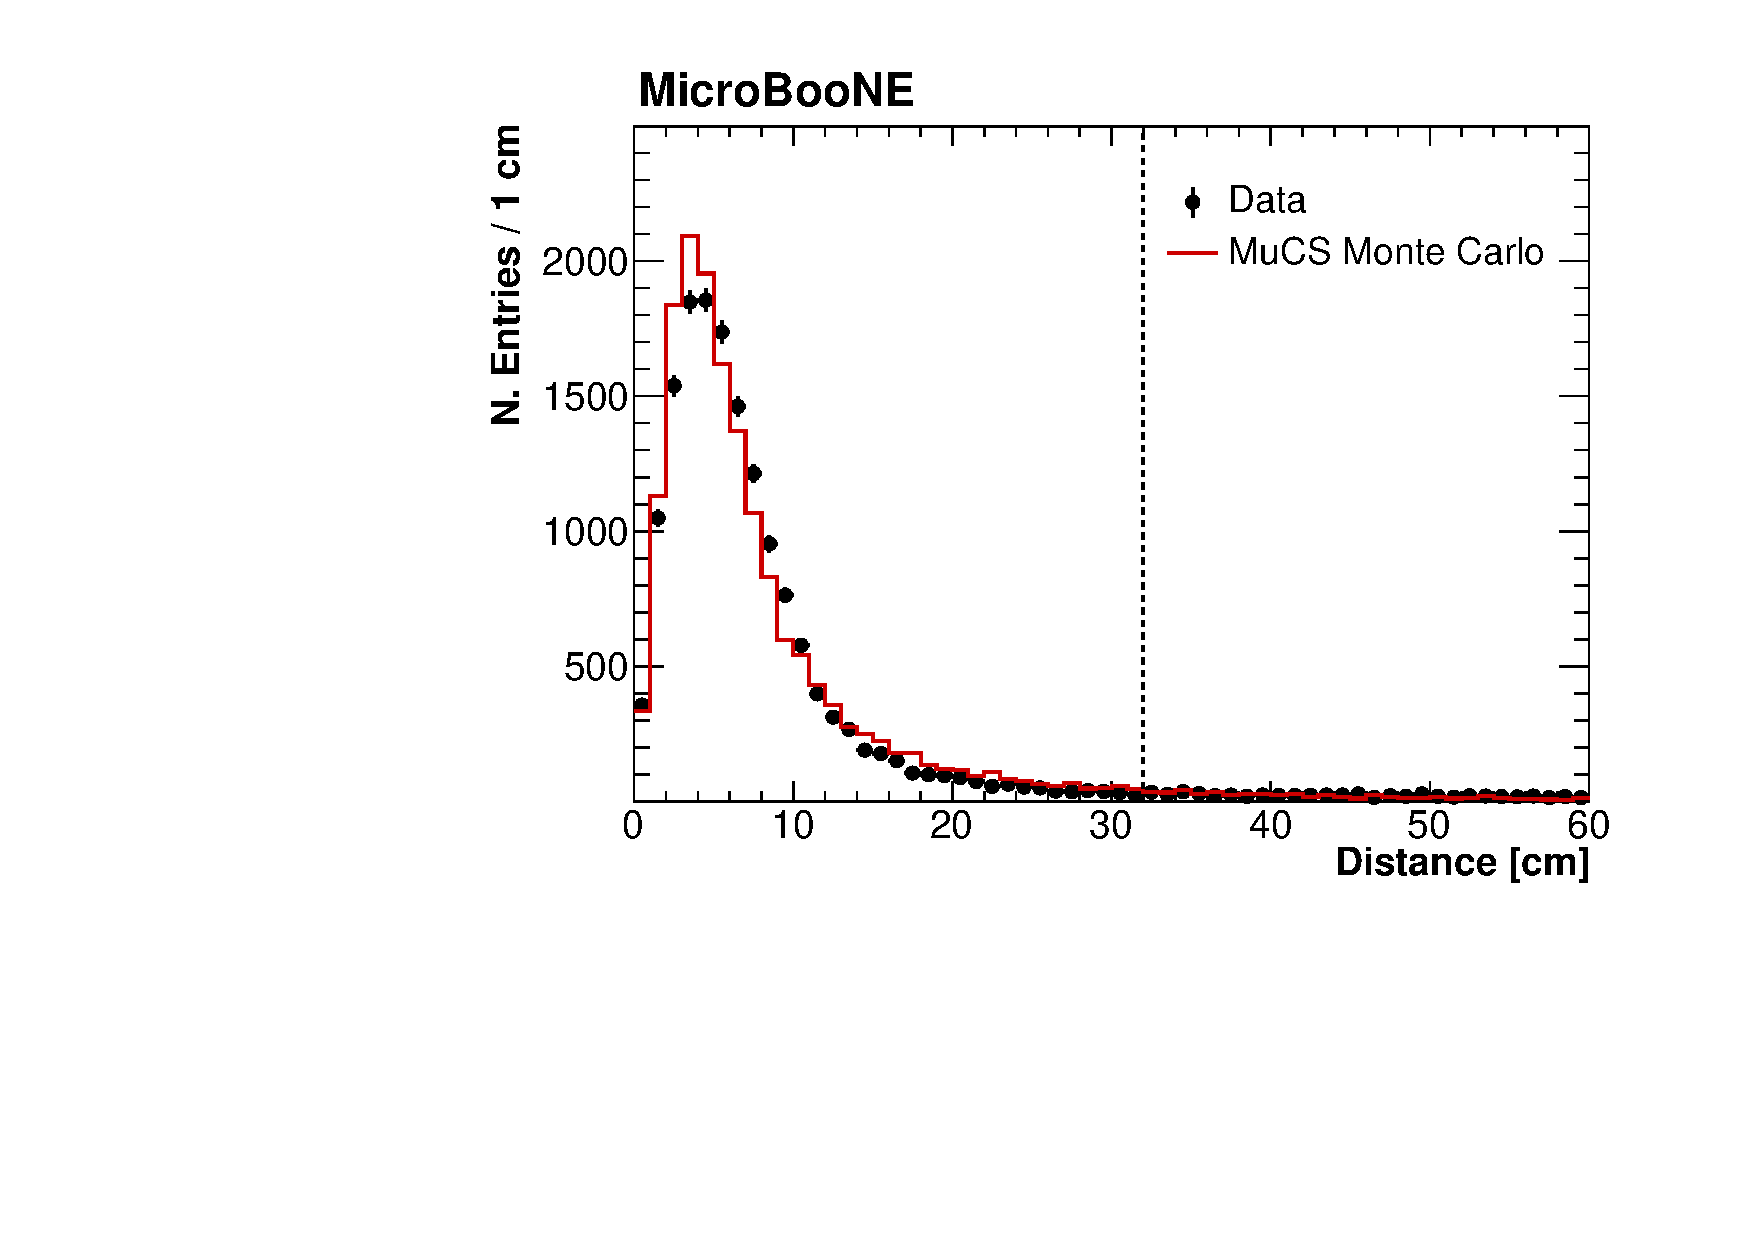
\includegraphics[width=0.7\linewidth]{figures/dist.pdf}
    \caption{Data and MuCS Monte Carlo distributions of the distance $d$ between the extrapolated starting point and the closest reconstructed starting point. The dashed line correspond to the chosen $d_{\mathrm{max}}$ cut (32 cm) for this analysis.} \label{fig:dist}
  \end{center}
\end{figure}

The efficiency $\epsilon_{\mathrm{tag}}$ of the cut on $d_{\mathrm{max}}$ is defined as:
\begin{equation}
  \epsilon_{\mathrm{tag}}=\frac{\mathrm{N.~of~events~with~a~reco.~cosmic~ray~within~}d_{\mathrm{max}}}{\mathrm{N.~of~MuCS~triggered~events}}.
\end{equation}
It can be calculated for the data sample ($\epsilon^{\mathrm{data}}_{\mathrm{tag}}$) and also for the MuCS Monte Carlo sample ($\epsilon^{\mathrm{MuCS-MC}}_{\mathrm{tag}}$), replacing the number of MuCS-triggered events with the number of simulated MuCS events.

The purity $P$ of the Monte Carlo MuCS sample, which represents the fraction of correctly tagged MuCS cosmic rays, is defined as the ratio between the number of events with a reconstructed MuCS cosmic ray correctly identified within $d_{\mathrm{max}}$ and the number of events with a reconstructed cosmic ray within $d_{\mathrm{max}}$ (MuCS-tagged cosmic rays):
\begin{equation}
  P=\frac{\mathrm{N.~of~events~with~a~reco.~MuCS~cosmic\myhyphen ray~within~}d_{\mathrm{max}}}{\mathrm{N.~of~events~with~a~reco.~cosmic~ray~within~}d_{\mathrm{max}}}.
\end{equation}
The acceptance $A$ of the cut on $d_{\mathrm{max}}$, which represents the portion of MuCS cosmic rays within $d_{\mathrm{max}}$, is defined as the ratio between the number of events with a reconstructed MuCS cosmic ray inside the $d_{\mathrm{max}}$ cut and the total number of events with a reconstructed MuCS cosmic ray:
\begin{equation}
  A=\frac{\mathrm{N.~of~events~with~a~reco.~MuCS~cosmic\myhyphen ray~within~}d_{\mathrm{max}}}{\mathrm{N.~of~events~with~a~reco.~MuCS~cosmic\myhyphen ray}}.
\end{equation}
The acceptance of the $d_{\mathrm{max}}$ cut is mainly affected by the multiple Coulomb scattering between the MuCS and the TPC.

The MuCS reconstruction efficiency as defined in \eqref{eq:eff}, can then be obtained, both for data ($\epsilon_{\mathrm{data}}$) and for MuCS Monte Carlo ($\epsilon_{\mathrm{MuCS\myhyphen MC}}$), by:
\begin{equation}\label{eq:mceff}
  \epsilon = \epsilon_{\mathrm{tag}} \times P / A.
\end{equation}
where the $P/A$ ratio can be taken only from the MuCS Monte Carlo simulation, while $\epsilon_{\mathrm{tag}}$ can be measured with the data, $\epsilon^{\mathrm{data}}_{\mathrm{tag}}$, or with the MuCS Monte Carlo simulation, $\epsilon^{\mathrm{MuCS\myhyphen MC}}_{\mathrm{tag}}$.

Figure \ref{fig:purity} shows the tagging efficiency both for data ($\epsilon^{\mathrm{data}}_{\mathrm{tag}}$) and MuCS Monte Carlo  ($\epsilon^{\mathrm{MuCS\myhyphen MC}}_{\mathrm{tag}}$), the purity $P$ and the acceptance $A$ as a function of $d_{\mathrm{max}}$. The MuCS reconstruction efficiencies for data ($\epsilon_{\mathrm{data}}$) and Monte Carlo ($\epsilon_{\mathrm{MuCS\myhyphen MC}}$) are also shown as a reference.

\begin{figure}[htbp]
  \begin{center}
    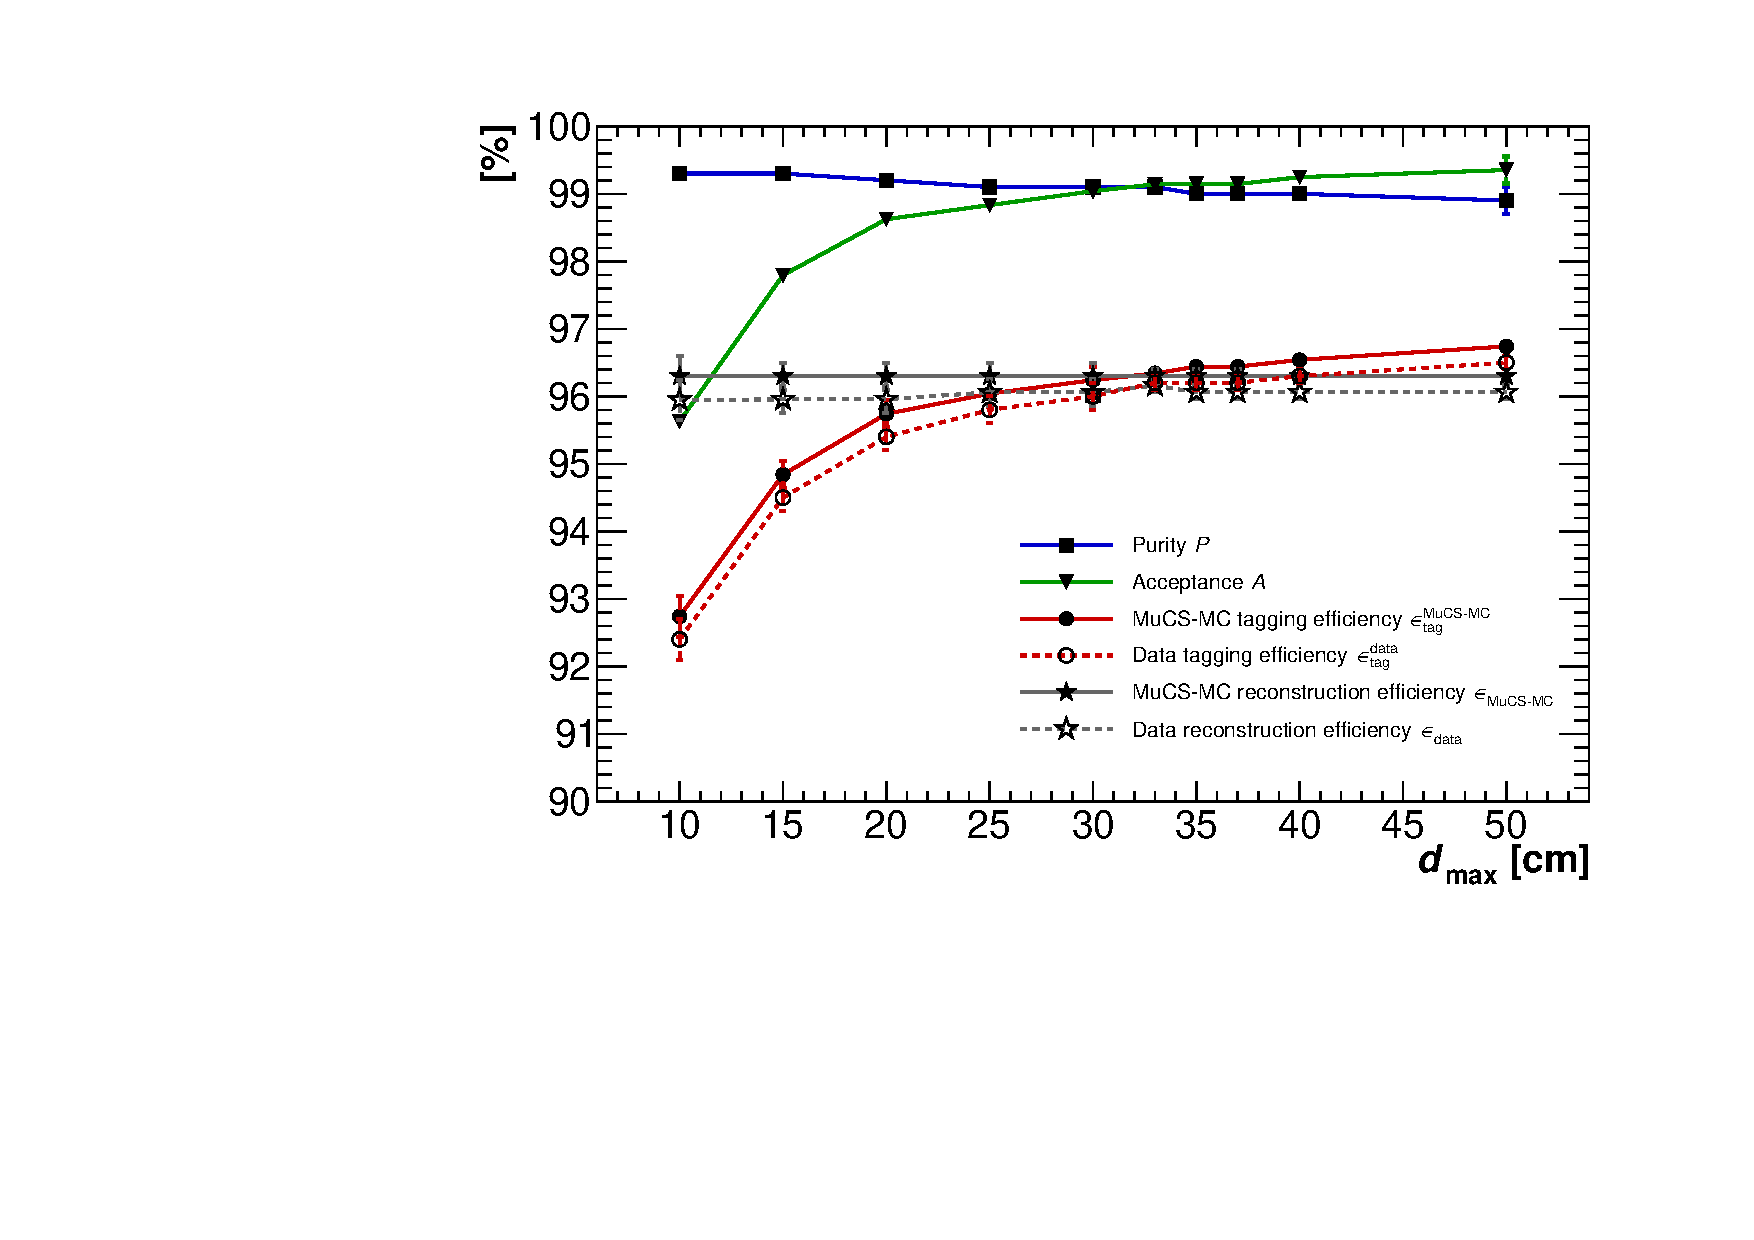
\includegraphics[width=0.7\linewidth]{figures/purity.pdf}
    \caption{Data ($\epsilon^{\mathrm{data}}_{\mathrm{tag}}$) and Monte Carlo ($\epsilon^{\mathrm{MC}}_{\mathrm{tag}}$) tagging efficiency (red), purity $P$ (blue) and acceptance $A$ (green), as a function of $d_{\mathrm{max}}$. The MuCS reconstruction efficiencies for data ($\epsilon_{\mathrm{data}}$) and MuCS Monte Carlo ($\epsilon_{\mathrm{MuCS\myhyphen MC}}$) are also shown as a reference (grey).} \label{fig:purity}
  \end{center}
\end{figure}

Using eq. \eqref{eq:eff}, the MuCS Monte Carlo reconstruction efficiency $\epsilon_{\mathrm{MuCS\myhyphen MC}}$ will not depend, by construction, on the chosen value of $d_{\mathrm{max}}$. Since the $P/A$ correcting factor is measured with a Monte Carlo simulation, the data reconstruction efficiency $\epsilon_{\mathrm{data}}$ will have a small dependence on $d_{\mathrm{max}}$ (see figure \ref{fig:purity}), because of the small difference between $\epsilon^{\mathrm{data}}_{\mathrm{tag}}$ and $\epsilon^{\mathrm{MuCS\myhyphen MC}}_{\mathrm{tag}}$.
The difference between the lowest and the highest value of $\epsilon_{\mathrm{data}}$ is 0.2\%. This value is used to quote the systematic uncertainty related to the $P/A$ correcting factor, as further discussed in section \ref{sec:sys}.
The chosen value of $d_{\mathrm{max}}$ is $d_{\mathrm{max}}=32~\mathrm{cm}$. Figure \ref{fig:dist} and figure \ref{fig:purity} show that around this value the $d$, $P$ and $A$ distributions are almost flat. For this particular value,  the ratio $P/A$ is 1.%, which is also a convenient choice for the calculation of $\epsilon_{\mathrm{data}}$.

% Values of $\epsilon_{\mathrm{data}}$ and $\epsilon_{\mathrm{MuCS\myhyphen MC}}$ for each configuration are reported in Tab. \ref{tab:config}.

% \begin{table}[htbp]
%   \centering
%   \begin{tabular}{lccccccccc}
%     \toprule
%     Configuration & \phantom{a} & \multicolumn{2}{c}{$\epsilon_{\mathrm{data}}$} & \phantom{a} & \multicolumn{2}{c}{$\epsilon_{\mathrm{MuCS\myhyphen MC}}$} \\
%      \cmidrule{3-4} \cmidrule{6-7}
%       &  & avg. & err. & & avg. & err.  \\
%     \midrule
%     Central & & 95.9 & 0.2 & & 96.3 & 0.1 \\
%     Upstream & & 95.7 & 0.2 & & 96.0 & 0.1 \\
%     Downstream & & 97.1 & 0.2 & & 97.3 & 0.1 \\
%     \midrule
%     Overall & & 96.1 & 0.1 & & 96.3 & 0.1 \\
%     \bottomrule
%   \end{tabular}
%   \caption{Reconstruction efficiency for each geometrical configuration for data and MuCS Monte Carlo.}\label{tab:config}
% \end{table}


The Monte Carlo cosmic-ray reconstruction efficiency, obtained with the Monte Carlo distribution generated as described in section \ref{sec:mcgen}, can be directly defined as:
\begin{equation}
  \epsilon_{\mathrm{MC}} = \frac{\mathrm{N.~of~reco.~cosmic\myhyphen ray~tracks}}{\mathrm{N.~of~generated~cosmic rays}}.
\end{equation}

This Monte Carlo sample contains cosmic rays generated all over the TPC, therefore  having an averaged any dependence of $\epsilon_{\mathrm{MC}}$ on the position of the cosmic ray in the TPC will be averaged out. The MuCS dataset, instead, covers only three regions of the detector, shown in figure \ref{fig:mucs}. A direct comparison of the MuCS data with the Monte Carlo sample allows to verify if the data reconstruction efficiency, measured in specific parts of the detector, is valid throughout the detector.

In an ideal TPC, the reconstruction efficiency for a cosmic ray depends only on the number of hit wires, which is given unequivocally by the direction and the length of the track in the TPC. In general, a cosmic ray with a longer path in the TPC will correspond to a larger number of hit wires, making it easier for the algorithm to reconstruct a track. The reconstruction efficiency depends also on the direction of the cosmic ray, since cosmic rays parallel with the wires of one plane (0, $\pm60^{\circ}$ with respect to the $y$ axis) will generate fewer hits in that particular plane, making the track reconstruction more difficult.
It is useful to express the data, $\epsilon_{\mathrm{data}}$, and the Monte Carlo, $\epsilon_{\mathrm{MC}}$, reconstruction efficiencies as a function of the spherical starting angles $\theta$, $\phi$ and of the expected track length $L$ in the TPC, as described in section \ref{sec:data_proc}.

The efficiency can then be plotted as a three-dimensional histogram: each bin will correspond to a particular combination of the $\theta$, $\phi$, $L$ variables. Bin width is chosen large enough to have a statistical efficiency error smaller than 10\% for every ($\theta$, $\phi$, $L$) bin. The same $P/A$ correction factor is applied to every bin. Figure \ref{fig:3d} shows both the data and the Monte Carlo reconstruction efficiency in that 3D phase space of $\theta$, $\phi$, $L$, calculated as described in section \ref{sec:merging}. The overall track reconstruction efficiency, obtained by integrating the three-dimensional histograms and considering only statistical uncertainties is:
\begin{align*}
\epsilon_{\mathrm{data}} &= 96.1 \pm 0.1~\%\\
\epsilon_{\mathrm{MC}} &= 97.3 \pm 0.1~\%
\end{align*} for data and Monte Carlo, respectively. However, this value of $\epsilon_{\mathrm{data}}$ does not take into account muons triggering the MuCS that decay or are captured before reaching the TPC. These events are counted in the denominator of eq. \eqref{eq:eff}, but they artificially lower the reconstruction efficiency since they haven't reached the TPC and cannot be reconstructed. The measurement and correction of this effect are described in detail in section \ref{sec:dif}.

\begin{figure}[htbp]
  \begin{subfigure}{0.52\textwidth}
    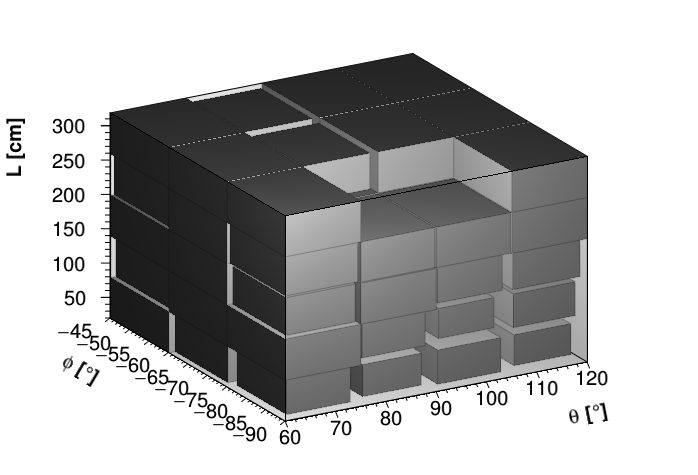
\includegraphics[width=\linewidth]{figures/3d_mc.png}
    \caption{Monte Carlo} \label{fig:3d_mc}
  \end{subfigure}
  \begin{subfigure}{0.52\textwidth}
    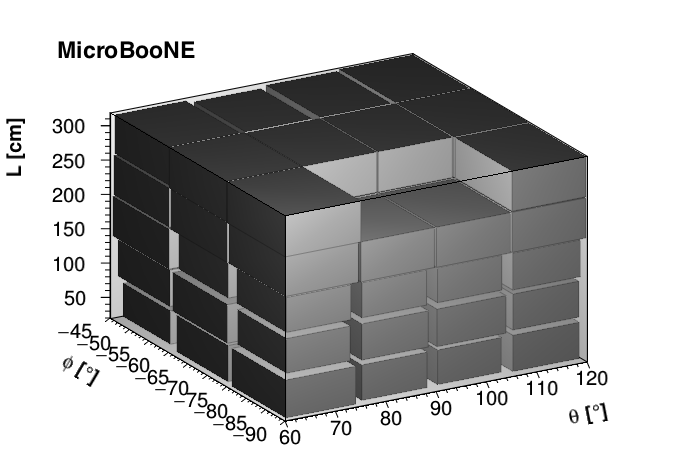
\includegraphics[width=\linewidth]{figures/3d_data.png}
    \caption{Data} \label{fig:3d_data}
  \end{subfigure}
  \caption{Monte Carlo and data three-dimensional reconstruction efficiency as a function of the starting angles $\theta$, $\phi$ and the extrapolated track length $L$. The size of the box represents the size of the efficiency. The empty region in the upper part of the plot corresponds to a region of the parameter space not covered by the data sample.}\label{fig:3d}
\end{figure}

\subsection{Systematic uncertainties}\label{sec:sys}
The measurement of the reconstruction efficiency can be affected by several systematic effects.
As shown in section \ref{sec:reco}, the value of $\epsilon_{\mathrm{data}}$ has a small dependence on the chosen value of $d_{\mathrm{max}}$. The difference between the highest and lowest value of $\epsilon_{\mathrm{data}}$, 0.2\%, has been taken as the systematic uncertainty relative to the $d_{\mathrm{max}}$ cut.

The number of reconstructed MuCS cosmic rays is normalized by the number of MuCS-triggered events, as shown in eq. \eqref{eq:eff}. However, some cosmic muon can decay or be stopped before reaching the TPC and they are then impossible to reconstruct. This systematic effect is described in section \ref{sec:dif}.

Moreover, since the data sample is measured in three specific parts of the detector, the presence of noisy or unresponsive wires could bias the measurement of the reconstruction efficiency. The systematic uncertainty related to this effect is evaluated in section \ref{sec:wires}.

The multiple Coulomb scattering of the cosmic ray in the material depends on the energy of the cosmic ray \cite{pdg}. Cosmic rays that scatter more have a higher probability to be outside the $d_{\mathrm{max}}$ cut and they are also more difficult to reconstruct. Thus, it can happen that in the ($\theta$, $\phi$, $L$) bins where the data reconstruction efficiency has been measured with low statistics, the MuCS cosmic rays can be distributed in a small region of the energy spectrum, which is very steep \cite{corsika}. This sampling effect could bias the measurement of the reconstruction efficiency. However,  this systematic effect has been verified to be negligible with the present level of statistics (smaller than 0.1\%).

\subsubsection{Decay-in-flight or captured muons}\label{sec:dif}
The cosmic muons hitting the MuCS can decay in flight or be captured before reaching the TPC. In this case, they trigger the MuCS but do not generate a cosmic track in the detector. Since in the definition of the data reconstruction efficiency $\epsilon_{\mathrm{data}}$, eq. \eqref{eq:eff}, the denominator corresponds to the number of MuCS-triggered events, and this effect needs to be corrected. The fraction $D$ of cosmic rays that go through the MuCS but decay or are captured before reaching the TPC has been measured from the MuCS Monte Carlo simulation as:
\begin{equation}
D = \frac{\mathrm{N.~of~decayed/captured~muons}}{\mathrm{N.~of~MuCS~triggered~events}} = 1.0 \pm 0.1~\%.
\end{equation}
This correction factor has been verified to be independent from $\theta$, $\phi$ and $L$. The corrected data reconstruction efficiency is given by:
\begin{equation}
\epsilon_{\mathrm{data}}^{\mathrm{corr}} =  \frac{\epsilon_{\mathrm{data}}}{1-D} = 97.1\%.
\end{equation}
The statistical uncertainty of the correcting factor $D$, 0.1\%, is considered as the systematic uncertainty related to this correction.

\subsubsection{Detector non-uniformities}\label{sec:wires}
A potential presence of detector non-uniformities can introduce a systematic uncertainty in the measurement of the reconstruction efficiency. In particular, the presence of noisy or unresponsive wires in specific regions of the detector can lower the reconstruction efficiency in some of the three datasets. However, the three different MuCS configurations (shown in figure \ref{fig:mucs}) allow to cover different regions of the TPC, providing information on potential non-uniformities.

To check if these non-uniformities introduce a systematic effect, the significance $\sigma$ of the differences between the data reconstruction efficiencies measured in two different configurations with the following definition has been calculated:
\begin{equation}
\sigma = \frac{\epsilon_a-\epsilon_b}{\sqrt{\Delta \epsilon_{a}^2 + \Delta \epsilon_b^2}},
\end{equation}
where $\epsilon_{a}$ ($\epsilon_{b}$) is the reconstruction efficiency in the arbitrary $a$ ($b$) configuration and $\Delta \epsilon_{a}$ ($\Delta \epsilon_{b}$) is the corresponding statistical error. This significance has been measured for each corresponding $\theta,\phi,L$ bin and for each possible combination of central, downstream and upstream configuration (described in section \ref{sec:proc}). In presence of a systematic effect, the standard deviation of the significances distribution would be larger than unity. In this case, the Gaussian fit of the distribution gives $\sigma = 1.54\pm0.12$, suggesting detector non-uniformity.

% \begin{figure}[htbp]
%   \begin{center}
%     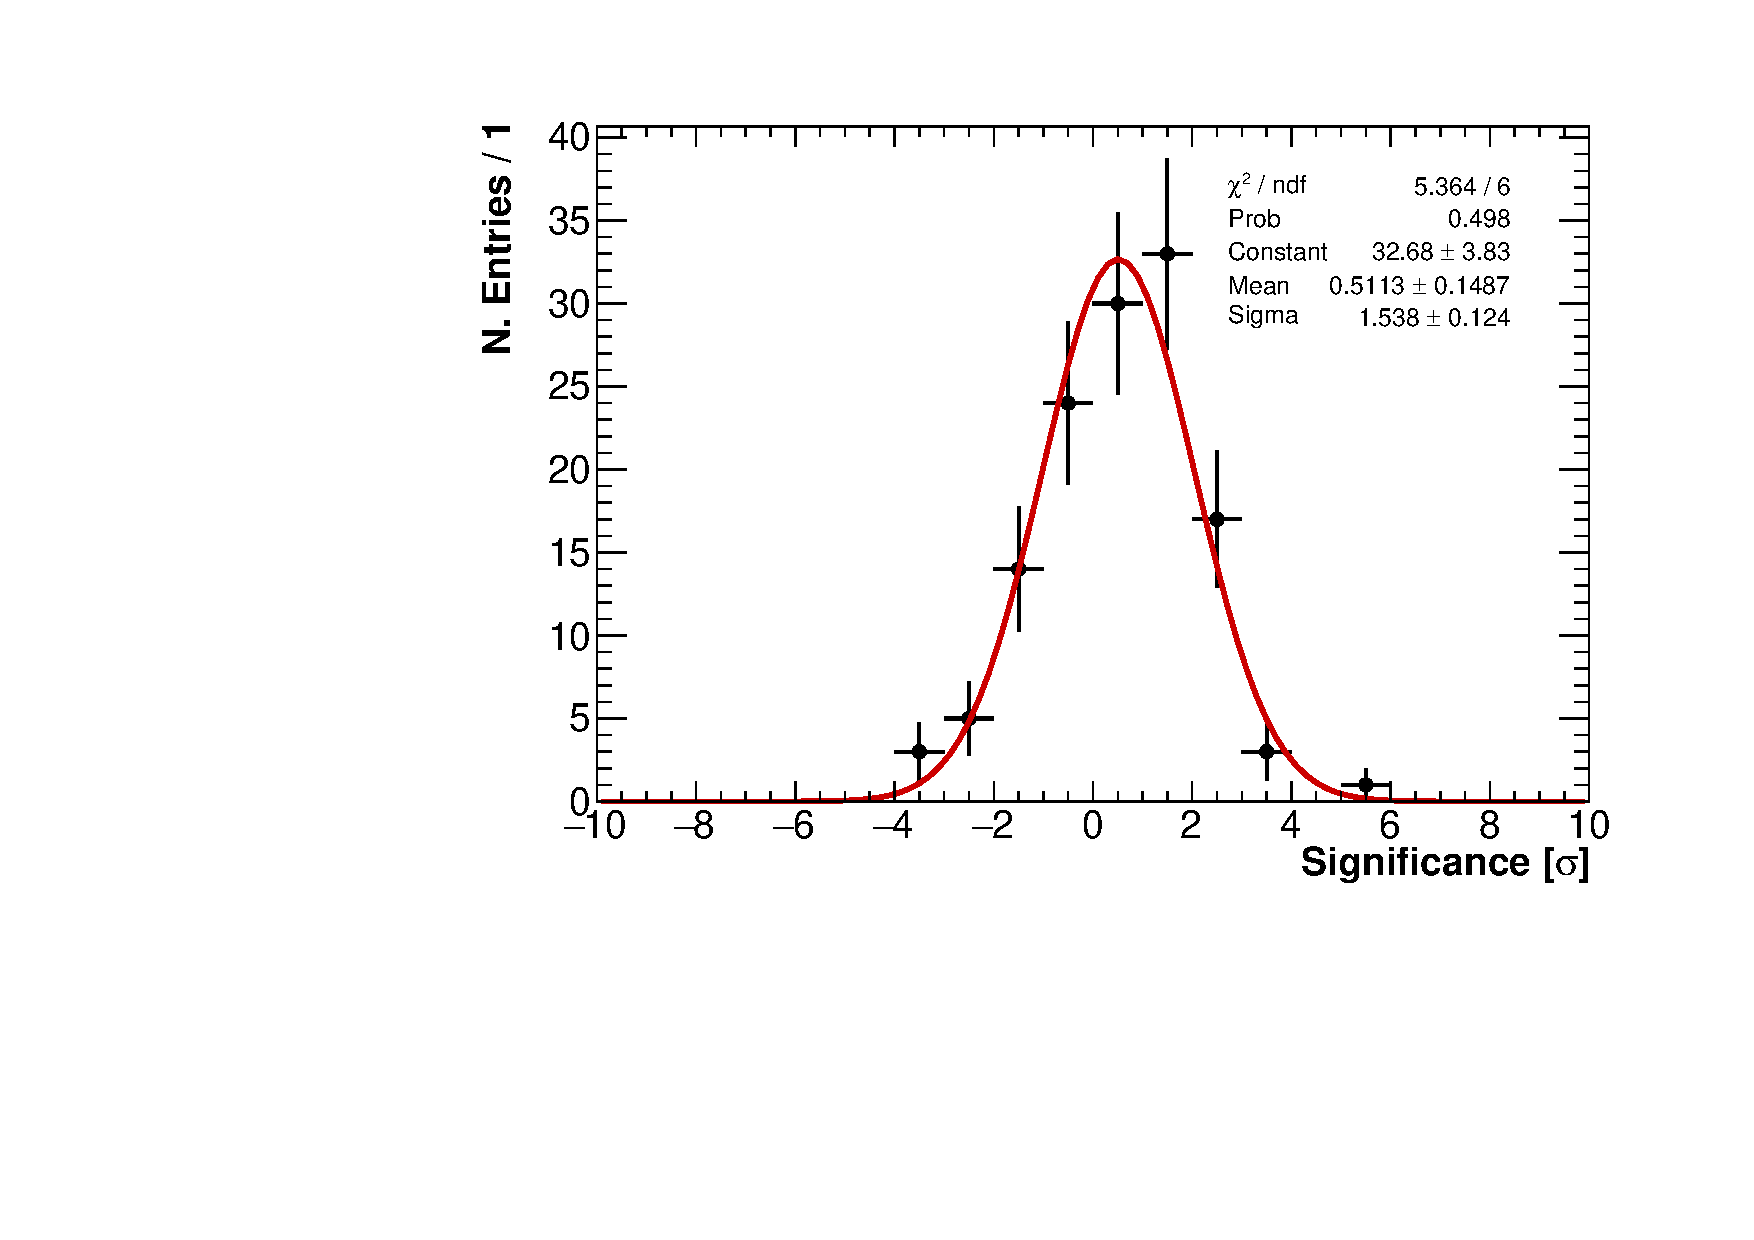
\includegraphics[width=0.7\linewidth]{figures/significance.pdf}
%     \caption{Distribution of the significances of the reconstruction efficiency for each $\theta,\phi,L$ bin, measured for any combination of the three MuCS configuration.} \label{fig:significance}
%   \end{center}
% \end{figure}

%In order to understand if these discrepancies are caused by noisy or unresponsive wires in specific parts of detector, the bins corresponding to significances larger than 3 have been reported in Tab. \ref{tab:significance}.

% \begin{table}[htbp]
%   \centering
%   \begin{tabular}{cccccccccccc}
%     \toprule
%     $\theta\thinspace[^\circ]$ & $\phi\thinspace[^\circ]$ & $L\thinspace[\mathrm{cm}]$ & \phantom{a} & \multicolumn{2}{c}{Central} & \phantom{a} & \multicolumn{2}{c}{Upstream} & \phantom{a} & \multicolumn{2}{c}{Downstream}\\
%      \cmidrule{5-6} \cmidrule{8-9} \cmidrule{11-12}
%       &  &  & & avg. & err. & & avg. & err. & & avg. & err.   \\
%     \midrule
%     75 & -60 & 20 & & \textbf{0.85} & \textbf{0.04} & & \textbf{0.85} & \textbf{0.02} & & 0.95 & 0.02\\
%     90 & -90 & 140 & & 0.97 & 0.03 & & \textbf{0.70} & \textbf{0.07} & & 0.93 & 0.04\\
%     90 & -90 & 200 & & 0.99 & 0.01 & & \textbf{0.96} & \textbf{0.01} & & 0.99 & 0.01\\
%     90 & -60 & 140 & & 0.98 & 0.01 & & \textbf{0.96} & \textbf{0.01} & & 0.99 & 0.01\\
%     90 & -60 & 200 & & 0.99 & 0.01 & & \textbf{0.96} & \textbf{0.01} & & 0.89 & 0.01\\
%
%     \bottomrule
%   \end{tabular}
%   \caption{Reconstruction efficiency for each geometrical configuration with a difference significance larger than 3. The lowest value is reported in bold.}\label{tab:significance}
% \end{table}

 Cosmic rays corresponding to bins with a large $\sigma$ have been studied to find the source of the non-uniformities. The drawing of the MuCS-extrapolated tracks that correspond to bins with a significance larger than 3 shows that, for the upstream configuration, the corresponding cosmic rays go through regions with noisy or unresponsive wires in one of the induction planes (figure \ref{fig:wires}). In these cases, the configuration with the lowest reconstruction efficiency has been verified to be always the upstream one, pointing to the presence of missing or unresponsive wires in that regions as the source of the detector non-uniformities.

\begin{figure}[htbp]
  \begin{center}
    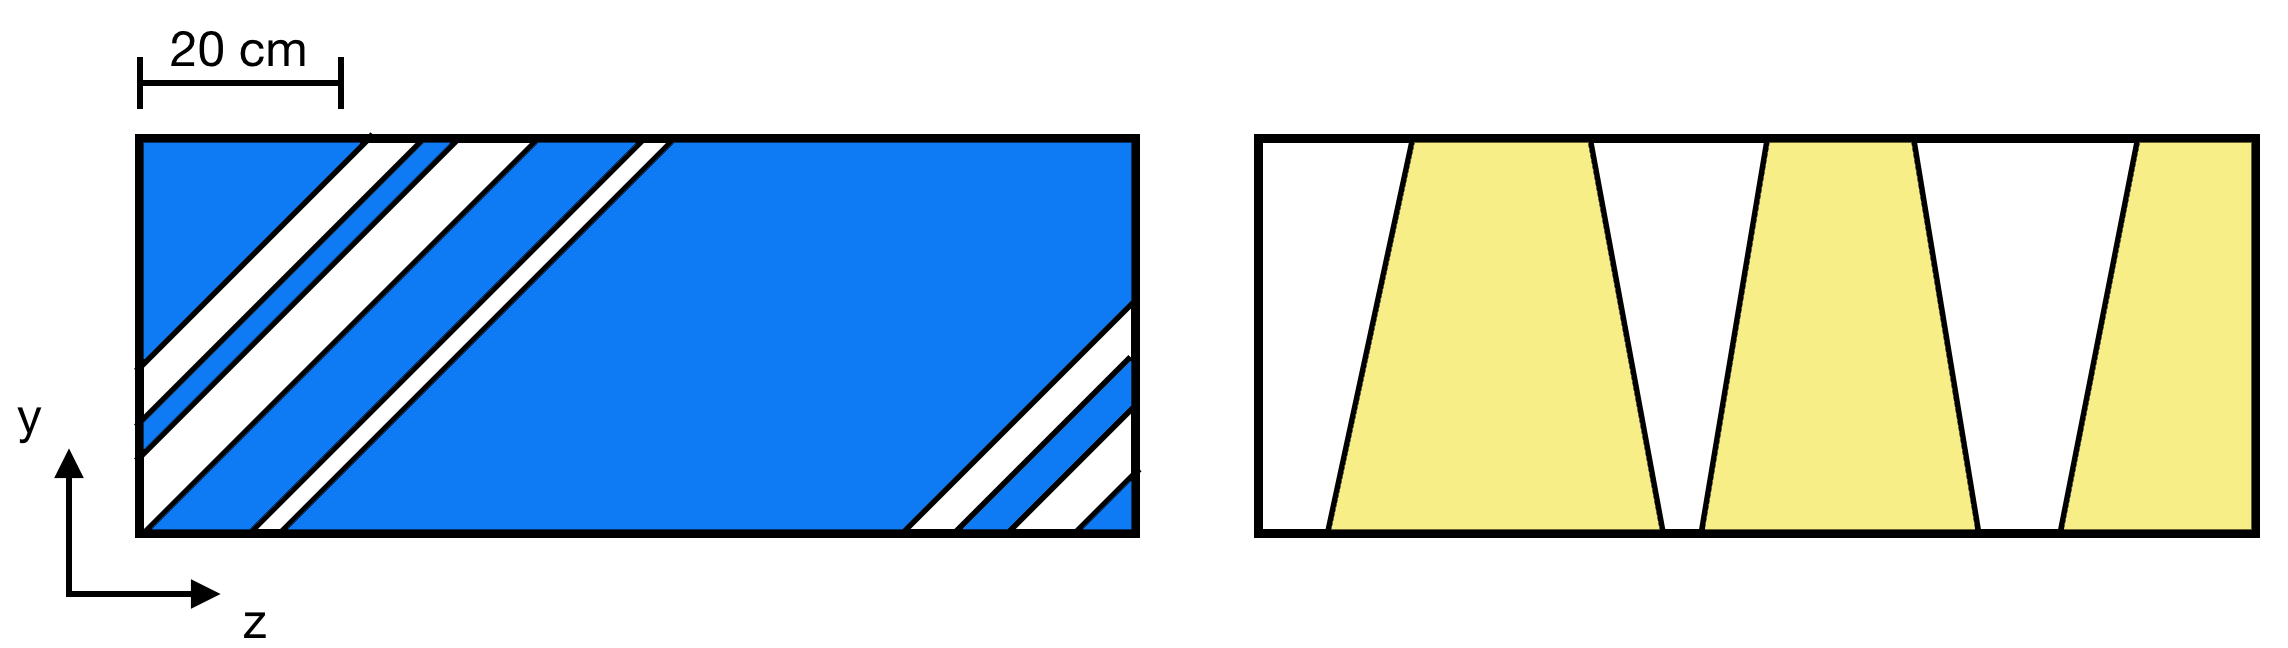
\includegraphics[width=1\linewidth]{figures/wire_tracks.png}
    \caption{Bi-dimensional plot of the collected charge during a cosmic-ray run, showing the regions with missing wires on one of the induction planes (left) and extrapolated tracks corresponding to bins with a significance larger than 3 (right). As shown by the picture on the right, the tracks in the upstream part of the detector (low $z$) go through a region with several missing wires.} \label{fig:wires}
  \end{center}
\end{figure}


Moreover, since the $\theta$ angle of the MuCS-extrapolated tracks is close to $90^\circ$, the cosmic rays in these bins are also aligned with the wires of the collection plane, parallel to the $y$ axis. Thus, the corresponding tracks have few hits in two of the three planes and the algorithm is not able to reconstruct them. Figure \ref{fig:example} shows the event display of a non-reconstructed MuCS cosmic ray going through the region with missing wires and parallel to the collection plane wires.

\begin{figure}[htbp]
  \begin{center}
    \begin{subfigure}{0.3\textwidth}
      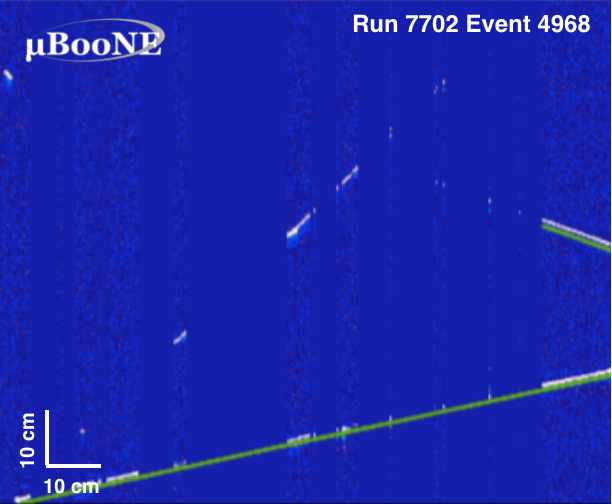
\includegraphics[width=\linewidth]{figures/u.png}
      \caption{Induction (U) plane} \label{fig:u}
    \end{subfigure}
    \begin{subfigure}{0.3\textwidth}
      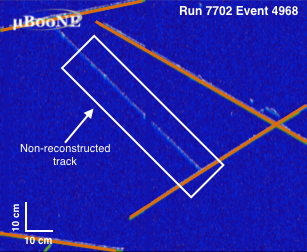
\includegraphics[width=\linewidth]{figures/v.png}
      \caption{Induction (V) plane} \label{fig:v}
    \end{subfigure}
    \begin{subfigure}{0.3\textwidth}
      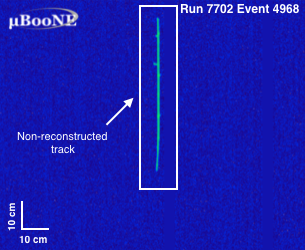
\includegraphics[width=\linewidth]{figures/y.png}
      \caption{Collection (Y) plane} \label{fig:y}
    \end{subfigure}    \caption{Event display of a non-reconstructed MuCS cosmic-ray track in the U, V and Y planes. Green lines correspond to the reconstructed tracks. The collection plane (Y) shows no reconstructed tracks.} \label{fig:example}
  \end{center}
\end{figure}

The systematic uncertainty related to the detector non-uniformities for each $\theta,\phi,L$ bin is quoted as the difference between the best reconstruction efficiency of the three configurations and the overall reconstruction efficiency (obtained by merging the three datasets), a method described in \cite{besiii}. The overall systematic uncertainty, calculated as the difference between the overall reconstruction efficiency of the best configuration and the overall reconstruction efficiency of the merged data sample, is 1.1\%.


%\subsection{Energy sampling}
%The multiple Coulomb scattering depends on the energy of the cosmic ray. The angular dispersion $\theta_{0}$ of a cosmic muon can be, in fact, calculated by the relation, expressed in \cite{pdg}:
%\begin{equation}
%\theta_{0} = \frac{13.6~\mathrm{MeV}}{\beta c p}\sqrt{x/X_{0}}\left[1+0.038\thinspace\mathrm{ln}(x/X_0)\right],
%\end{equation}
%where $p$ and $\beta c$ are the momentum and velocity of the incident particle, and $x/X_0$ is the thickness of the scattering medium in radiation lengths.

%\begin{figure}[htbp]
%  \begin{center}
%    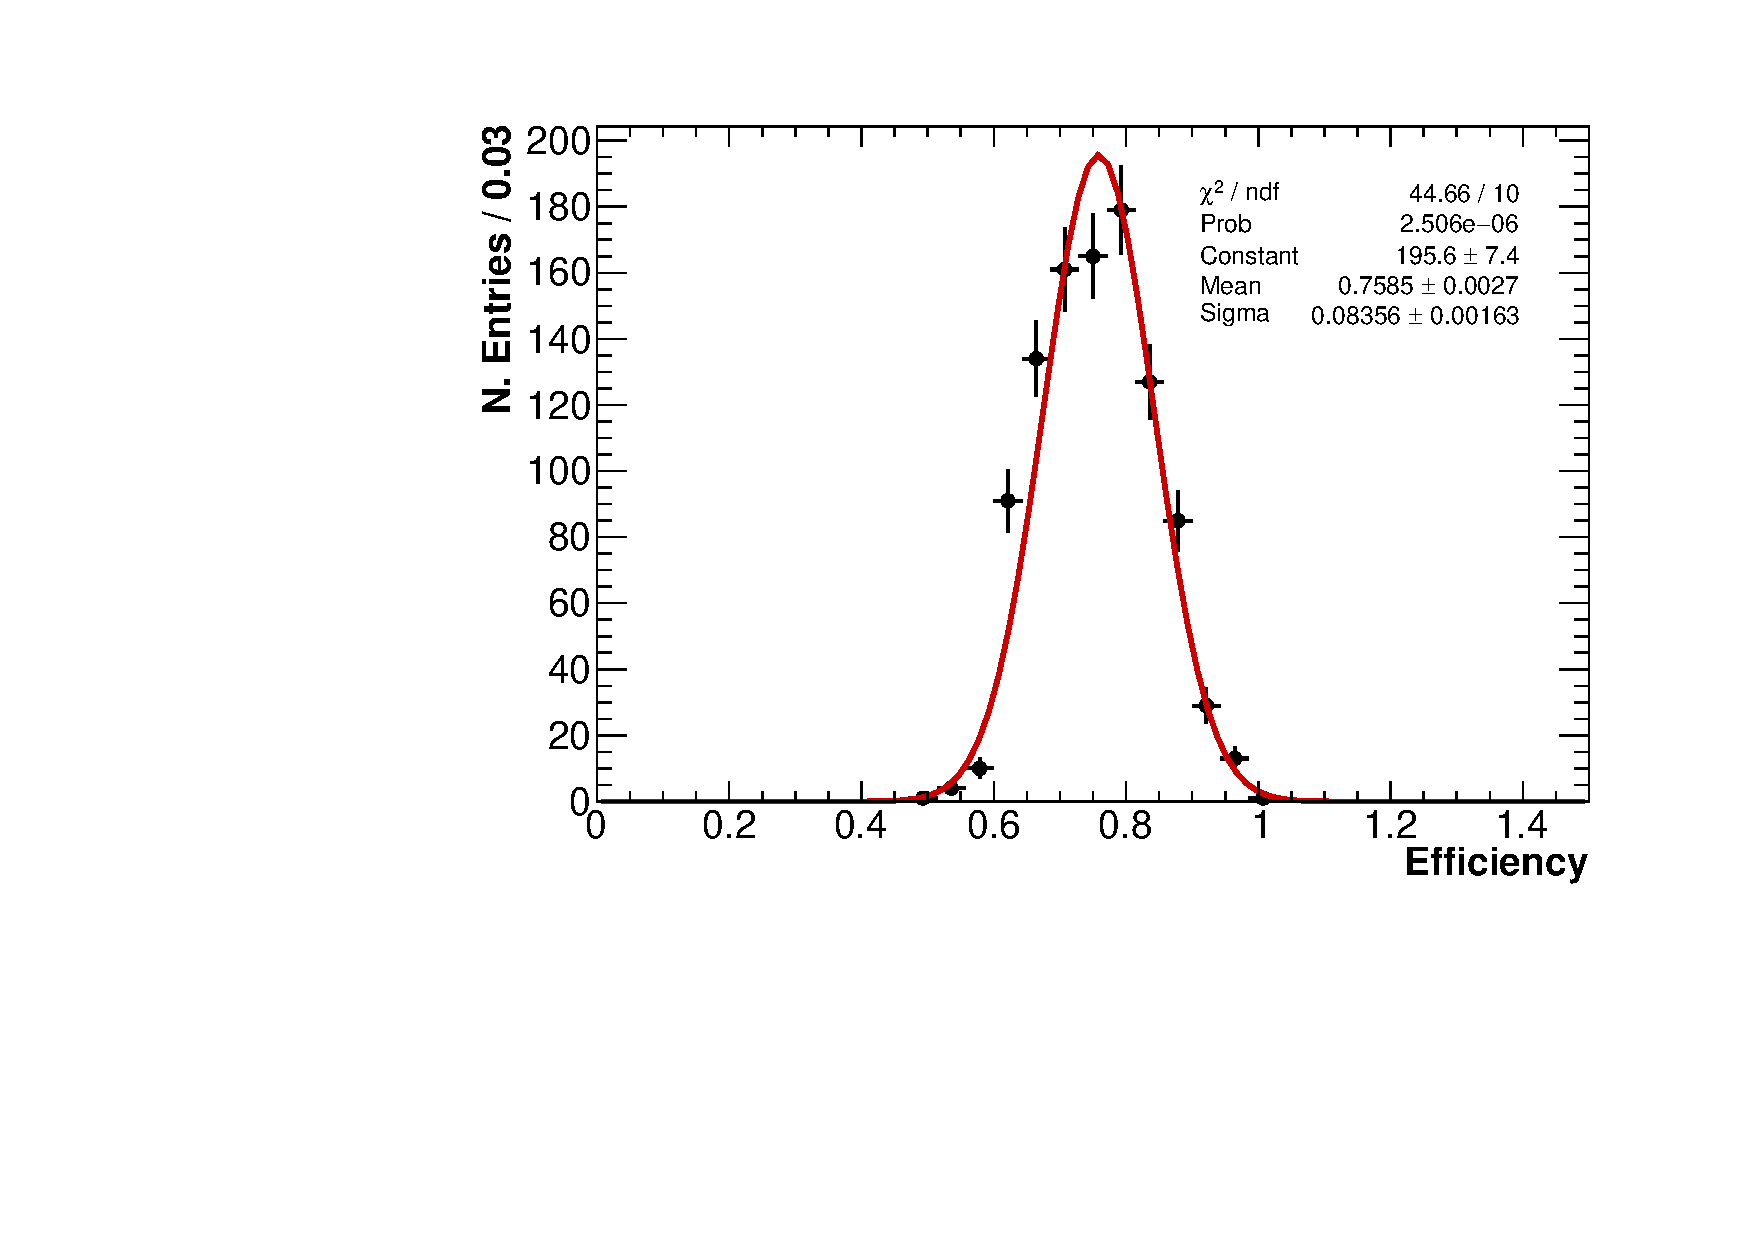
\includegraphics[width=0.7\linewidth]{figures/sampling.pdf}
%    \caption{Distribution of the reconstruction efficiency obtained generating 1000 thousand pseudo-experiments with 19 MuCS-triggered events each.} \label{fig:sampling}
%  \end{center}
%\end{figure}

%Thus, low-energy cosmic rays scatter more than high-energy ones and they have an higher probability to be further than $d_{\mathrm{max}}$ from the extrapolated starting point of the MuCS cosmic ray. In the bins where the data reconstruction efficiency has been measured with low statistics, then, it can happen to have MuCS cosmic rays distributed in a small region of the energy spectrum, biasing the measurement of the reconstruction efficiency.

%In order to verify if this sampling introduces a systematic effect, we choose the bin with the lowest number of MuCS events, which is 19. We then performed a Monte Carlo simulation, generating one thousand pseudo-experiments with 19 MuCS events sampled from the CORSIKA cosmic-ray energy spectrum with the same starting angles and length of our chosen bin. We filled a histogram with the value of the reconstruction efficiency for each pseudo-experiment and fitted the distribution with a Gaussian (figure \ref{fig:sampling}). The $\sigma$ of the fit is $0.084$, compatible with the statistical error of the same bin which is $0.083$. Thus, we conclude that the energy sampling of the cosmic rays does not introduce a systematic effect.

\subsection{Data/Monte Carlo comparison}\label{sec:datamc}
The reconstruction efficiencies have been calculated for Monte Carlo and data as described above. The data reconstruction efficiency has been corrected for the portion of cosmic muons decaying or being captured before reaching the TPC and can be compared with the Monte Carlo reconstructin efficiency.
For clarity, the three-dimensional efficiency plots shown in figure \ref{fig:3d} can be projected on the bi-dimensional planes ($\theta,\phi$), ($\theta,L$), ($\phi,L$), shown in figure \ref{fig:2d}, and on the single axis $\theta$, $\phi$, $L$, shown in figure \ref{fig:1d}.


\begin{figure}[htbp]
  \begin{subfigure}{0.33\textwidth}
    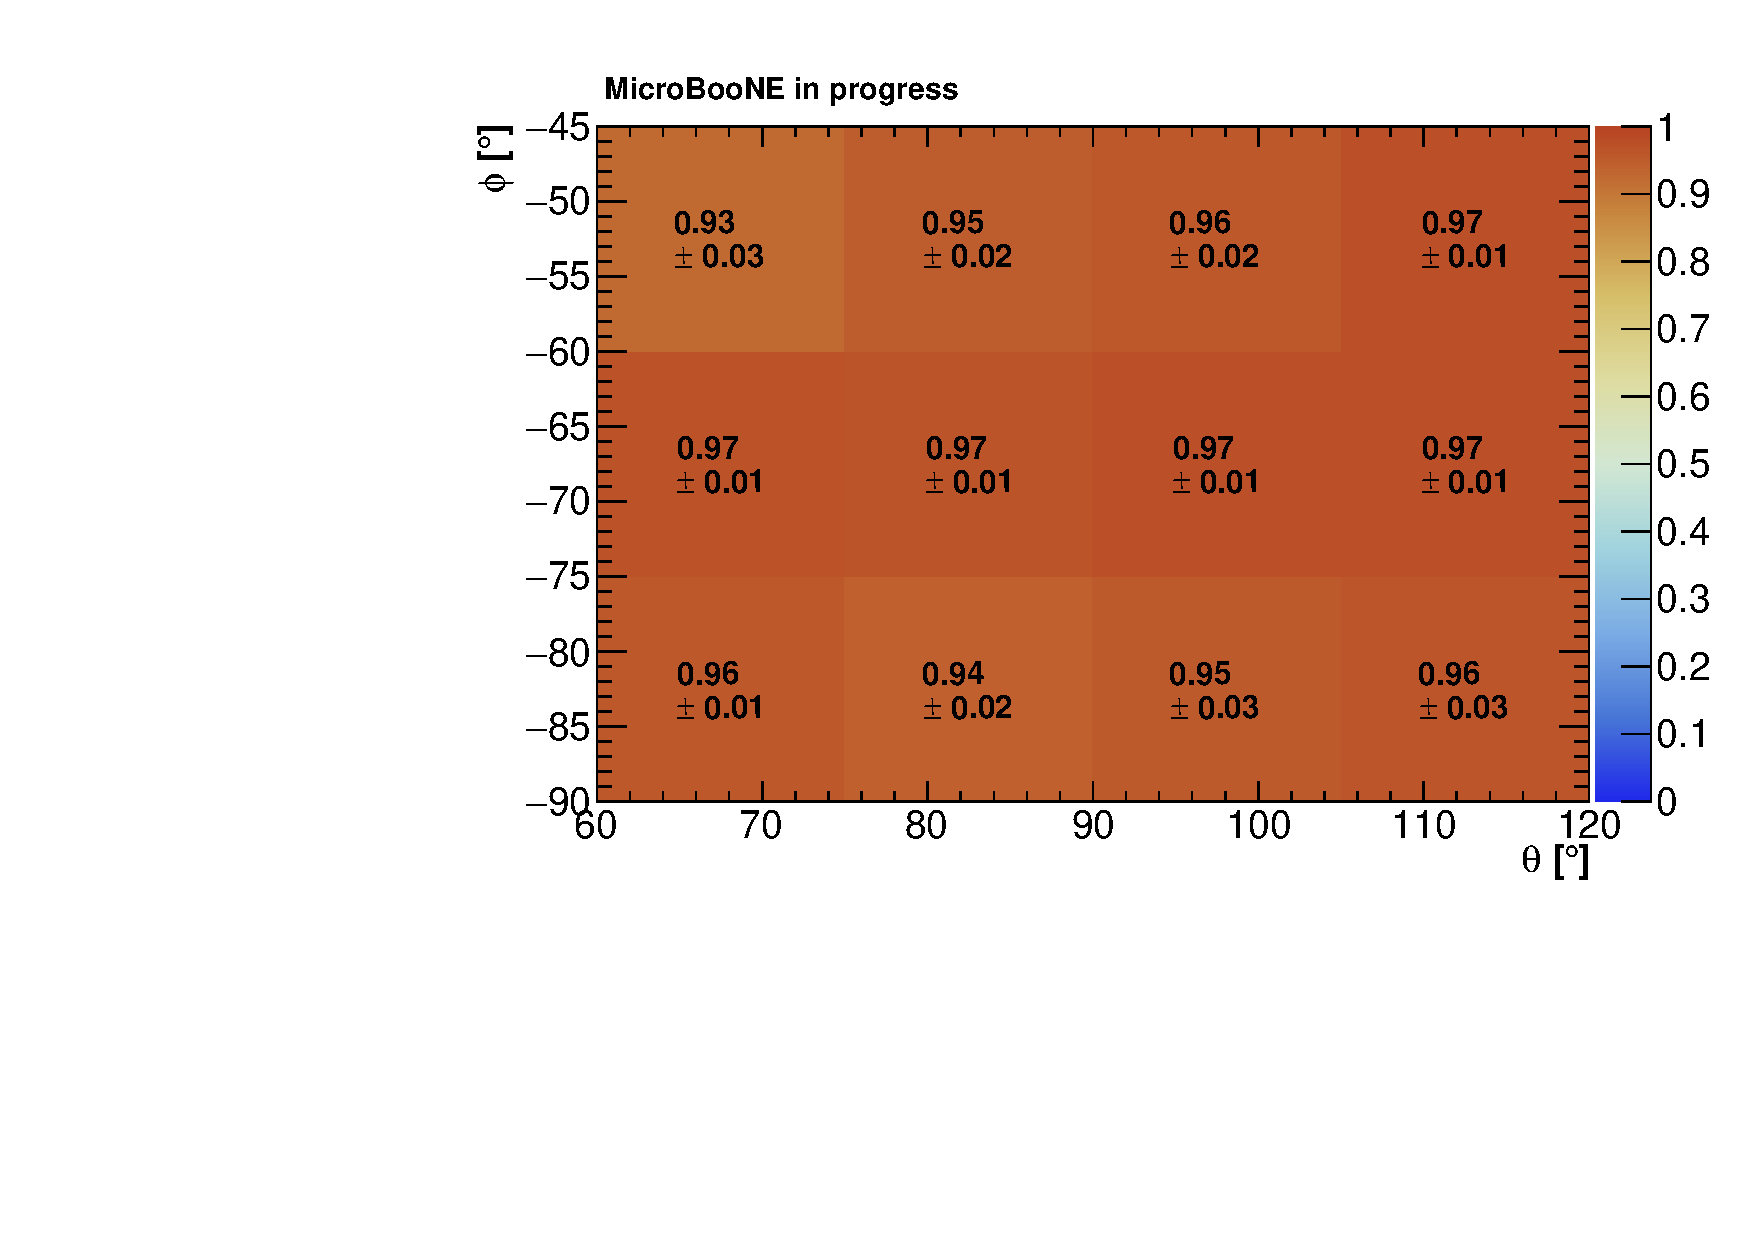
\includegraphics[width=\linewidth]{figures/e_theta_phi.pdf}
    \caption{$(\theta,\phi)$ - Data}
  \end{subfigure}\begin{subfigure}{0.33\textwidth}
  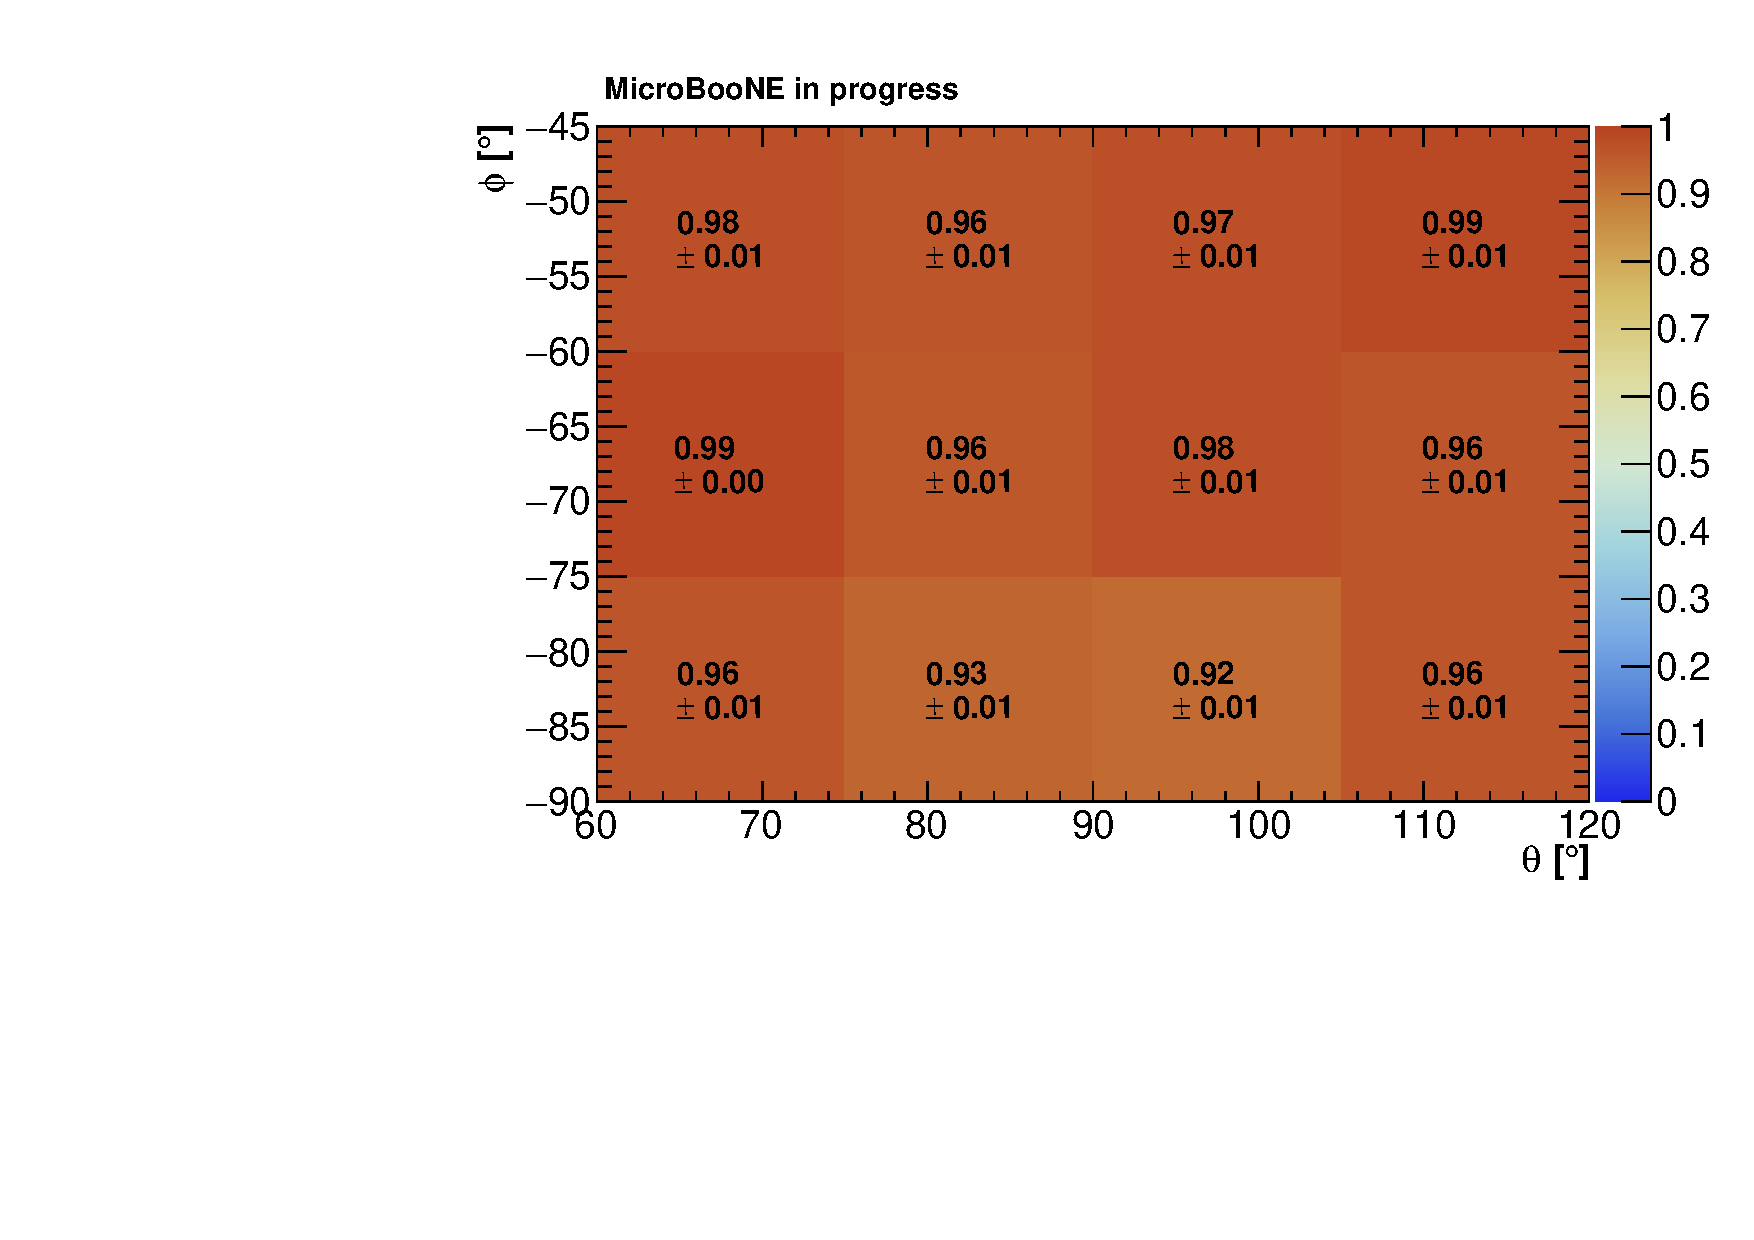
\includegraphics[width=\linewidth]{figures/theta_phi_mc.pdf}
  \caption{$(\theta,\phi)$ - Monte Carlo}
  \end{subfigure}\begin{subfigure}{0.33\textwidth}
  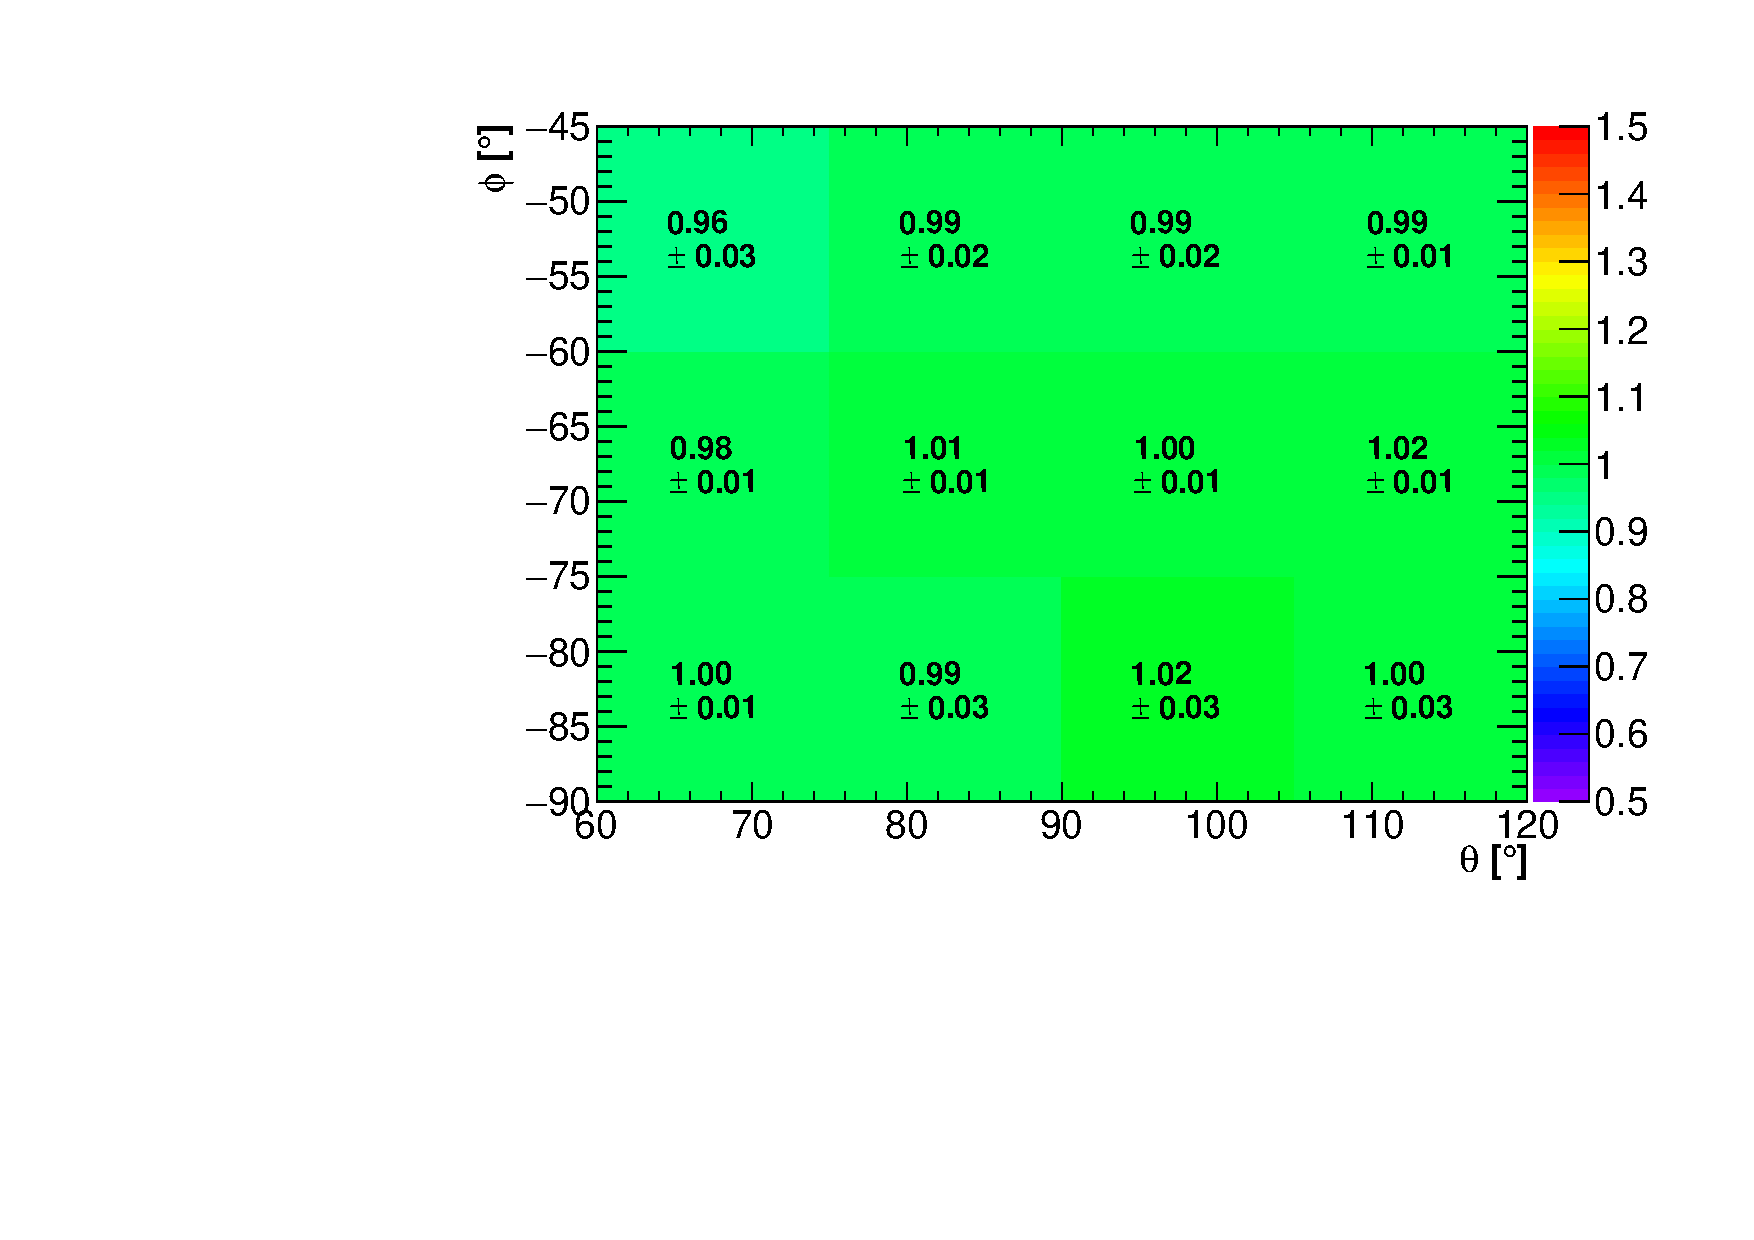
\includegraphics[width=\linewidth]{figures/theta_phi.pdf}
  \caption{$(\theta,\phi)$ - Data/Monte Carlo}
\end{subfigure}
\begin{subfigure}{0.33\textwidth}
  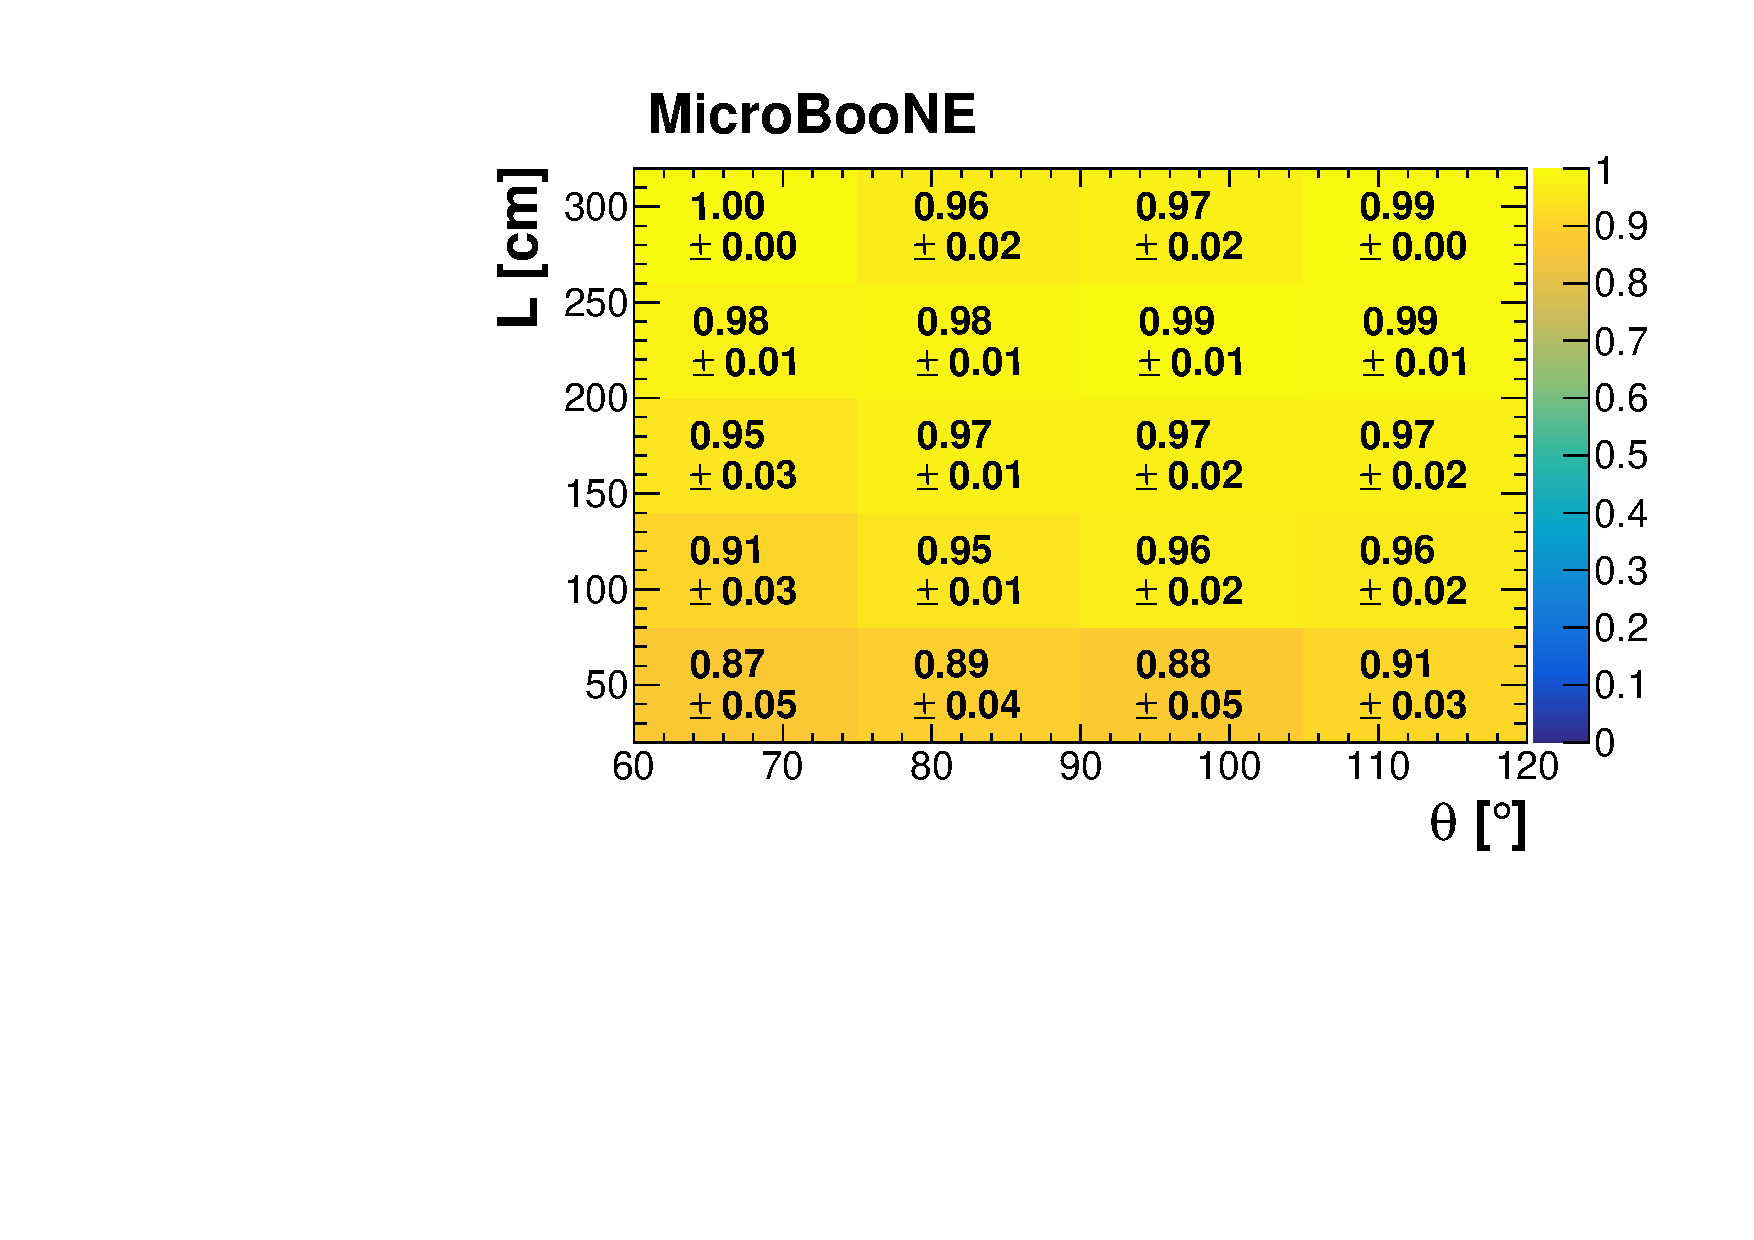
\includegraphics[width=\linewidth]{figures/e_theta_l.pdf}
  \caption{$(\theta,L)$ - Data}
\end{subfigure}\begin{subfigure}{0.33\textwidth}
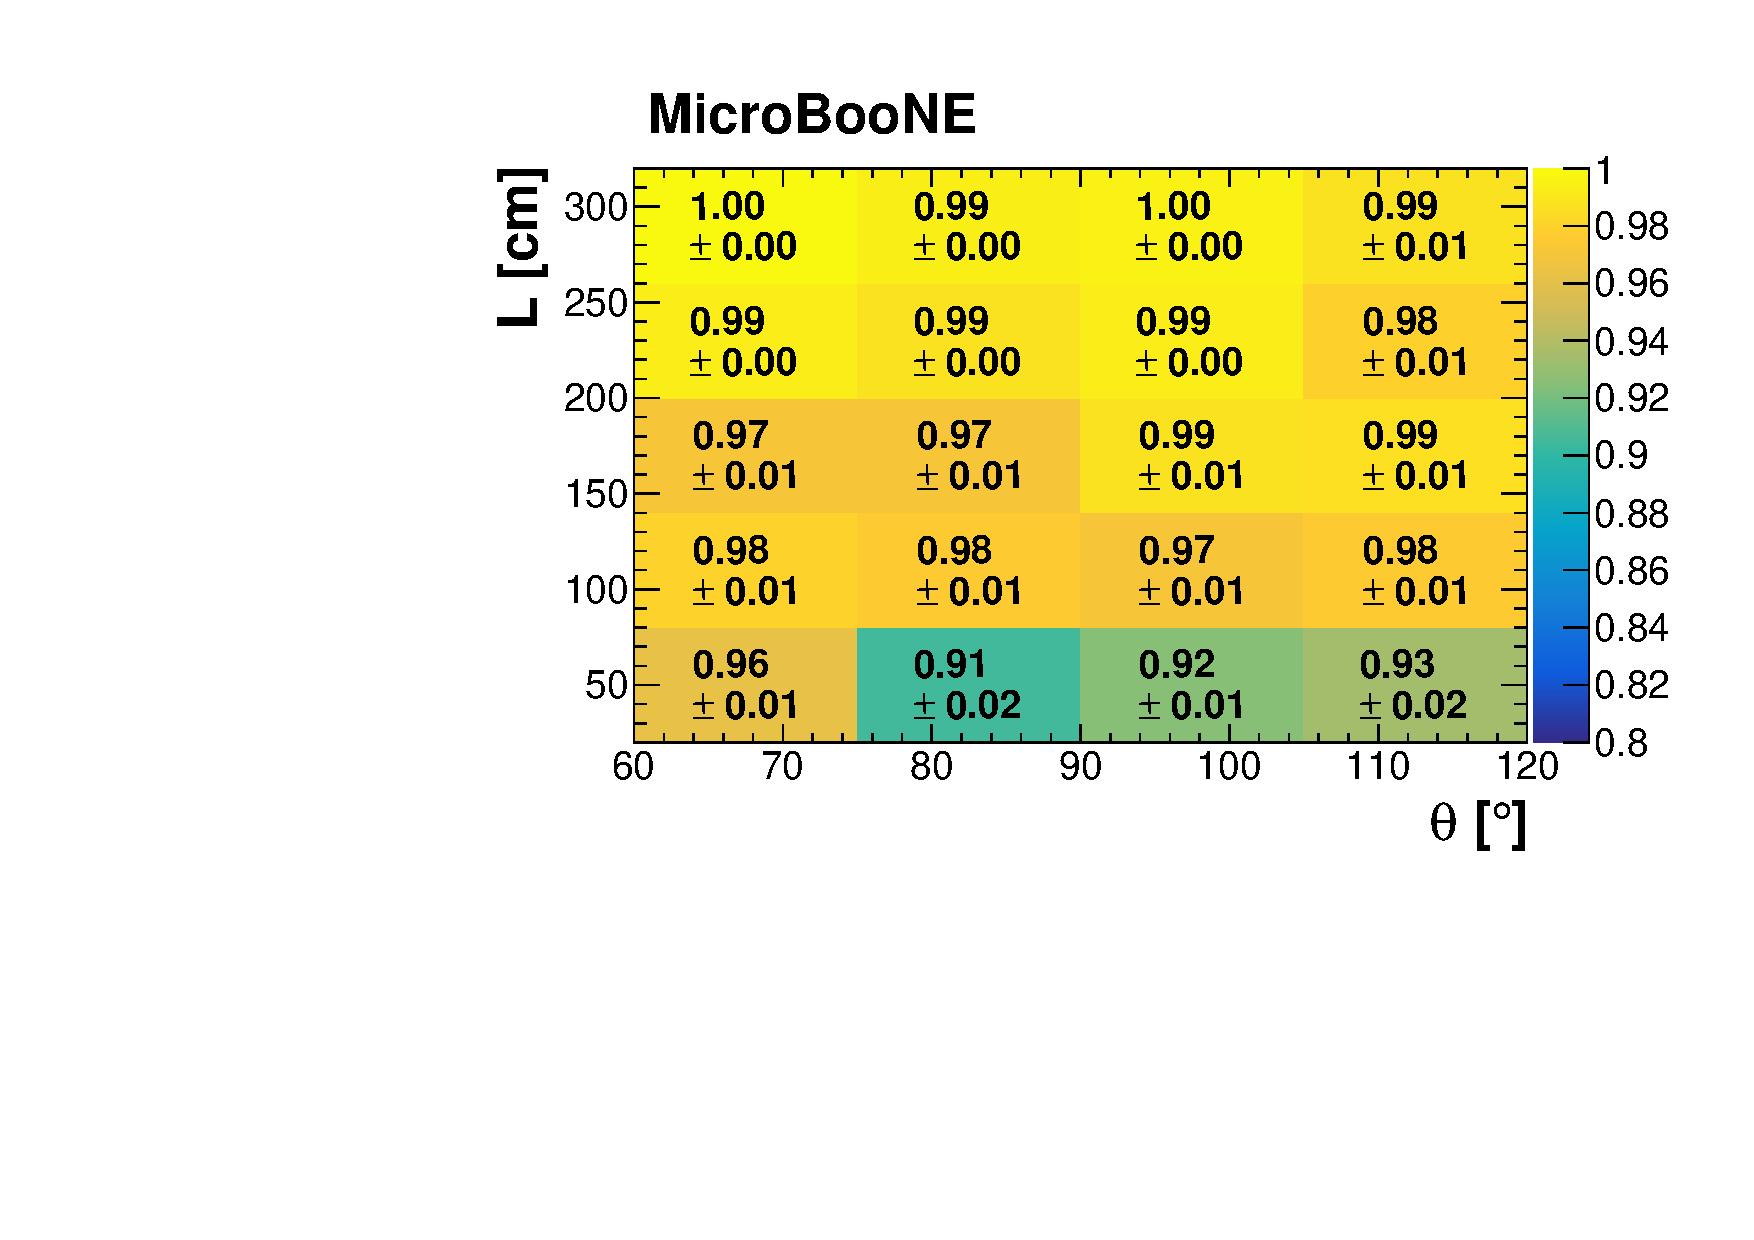
\includegraphics[width=\linewidth]{figures/theta_l_mc.pdf}
\caption{$(\theta,L)$ - Monte Carlo}
\end{subfigure}\begin{subfigure}{0.33\textwidth}
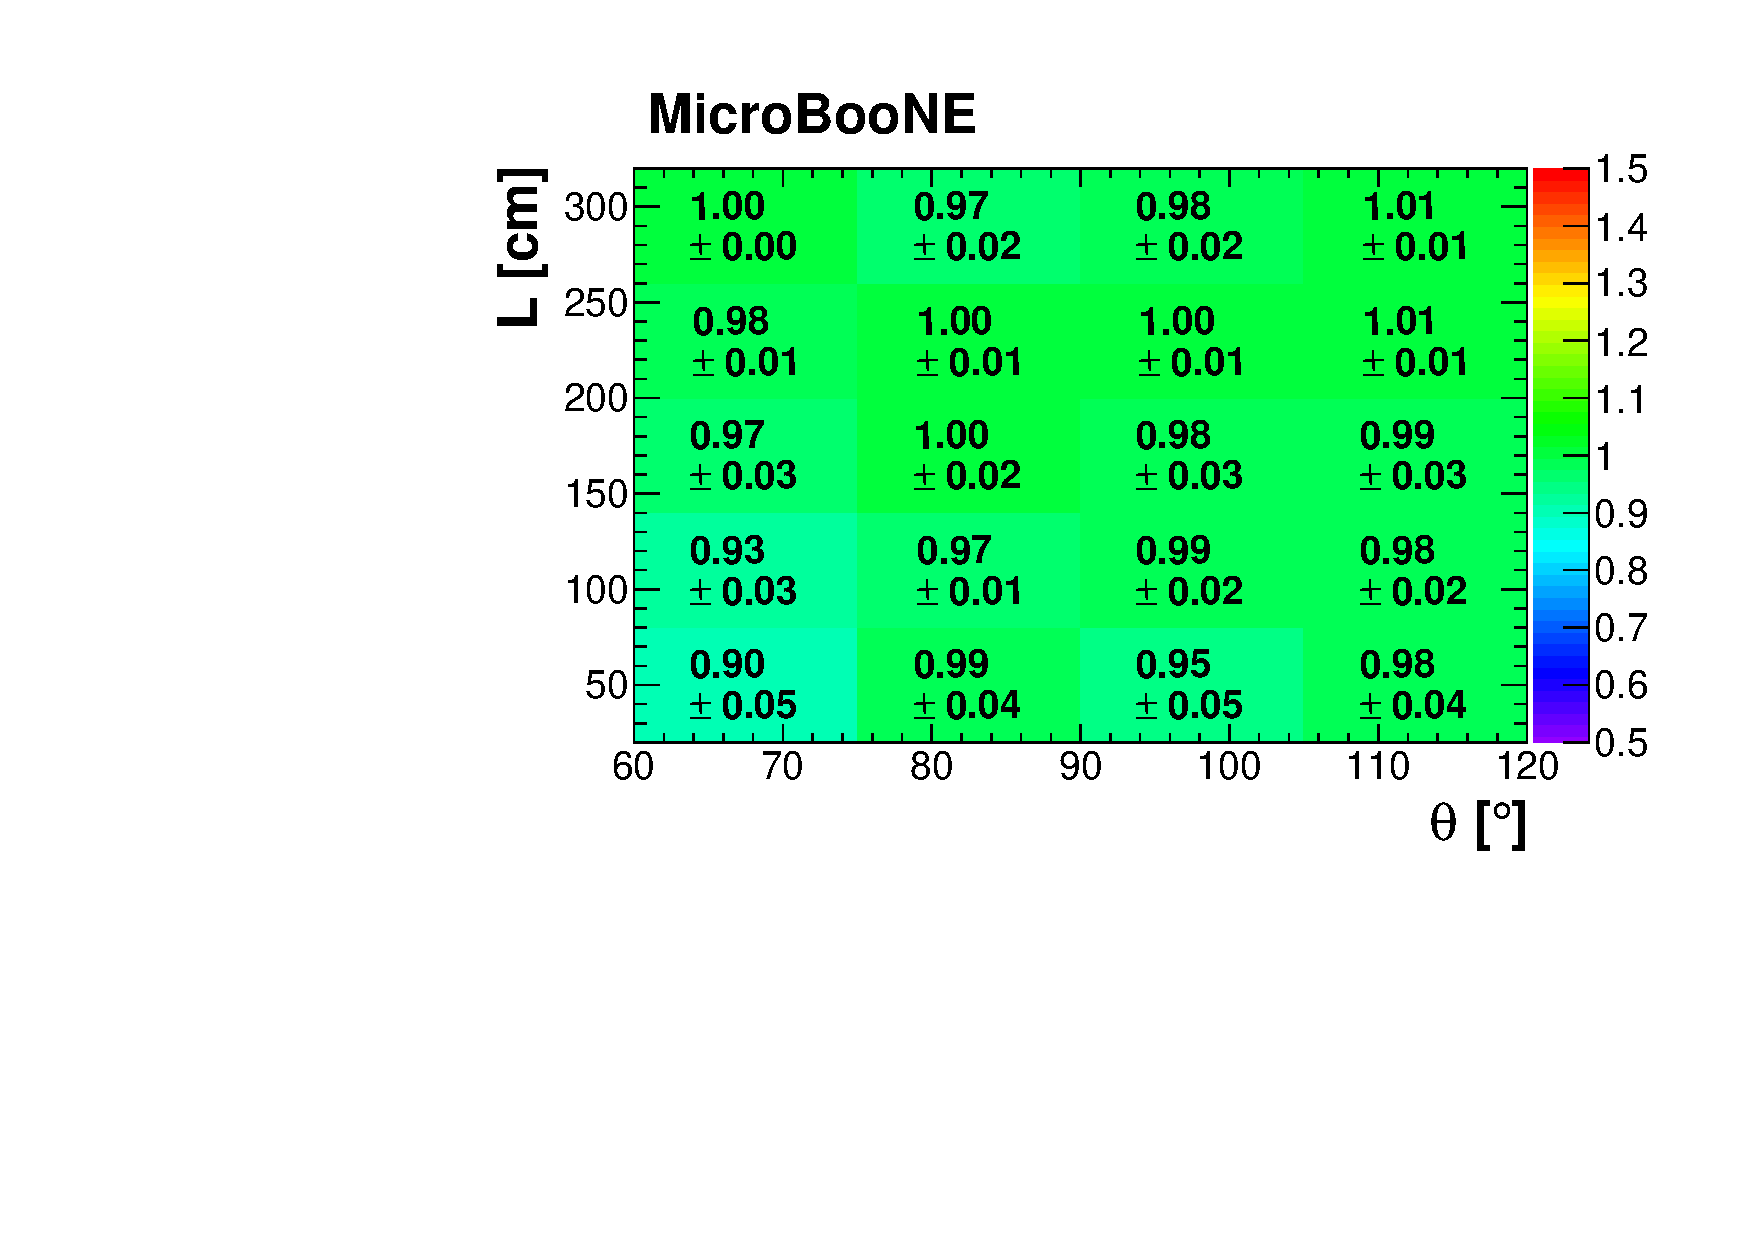
\includegraphics[width=\linewidth]{figures/theta_l.pdf}
\caption{$(\theta,L)$ - Data/Monte Carlo}
\end{subfigure}
\begin{subfigure}{0.33\textwidth}
  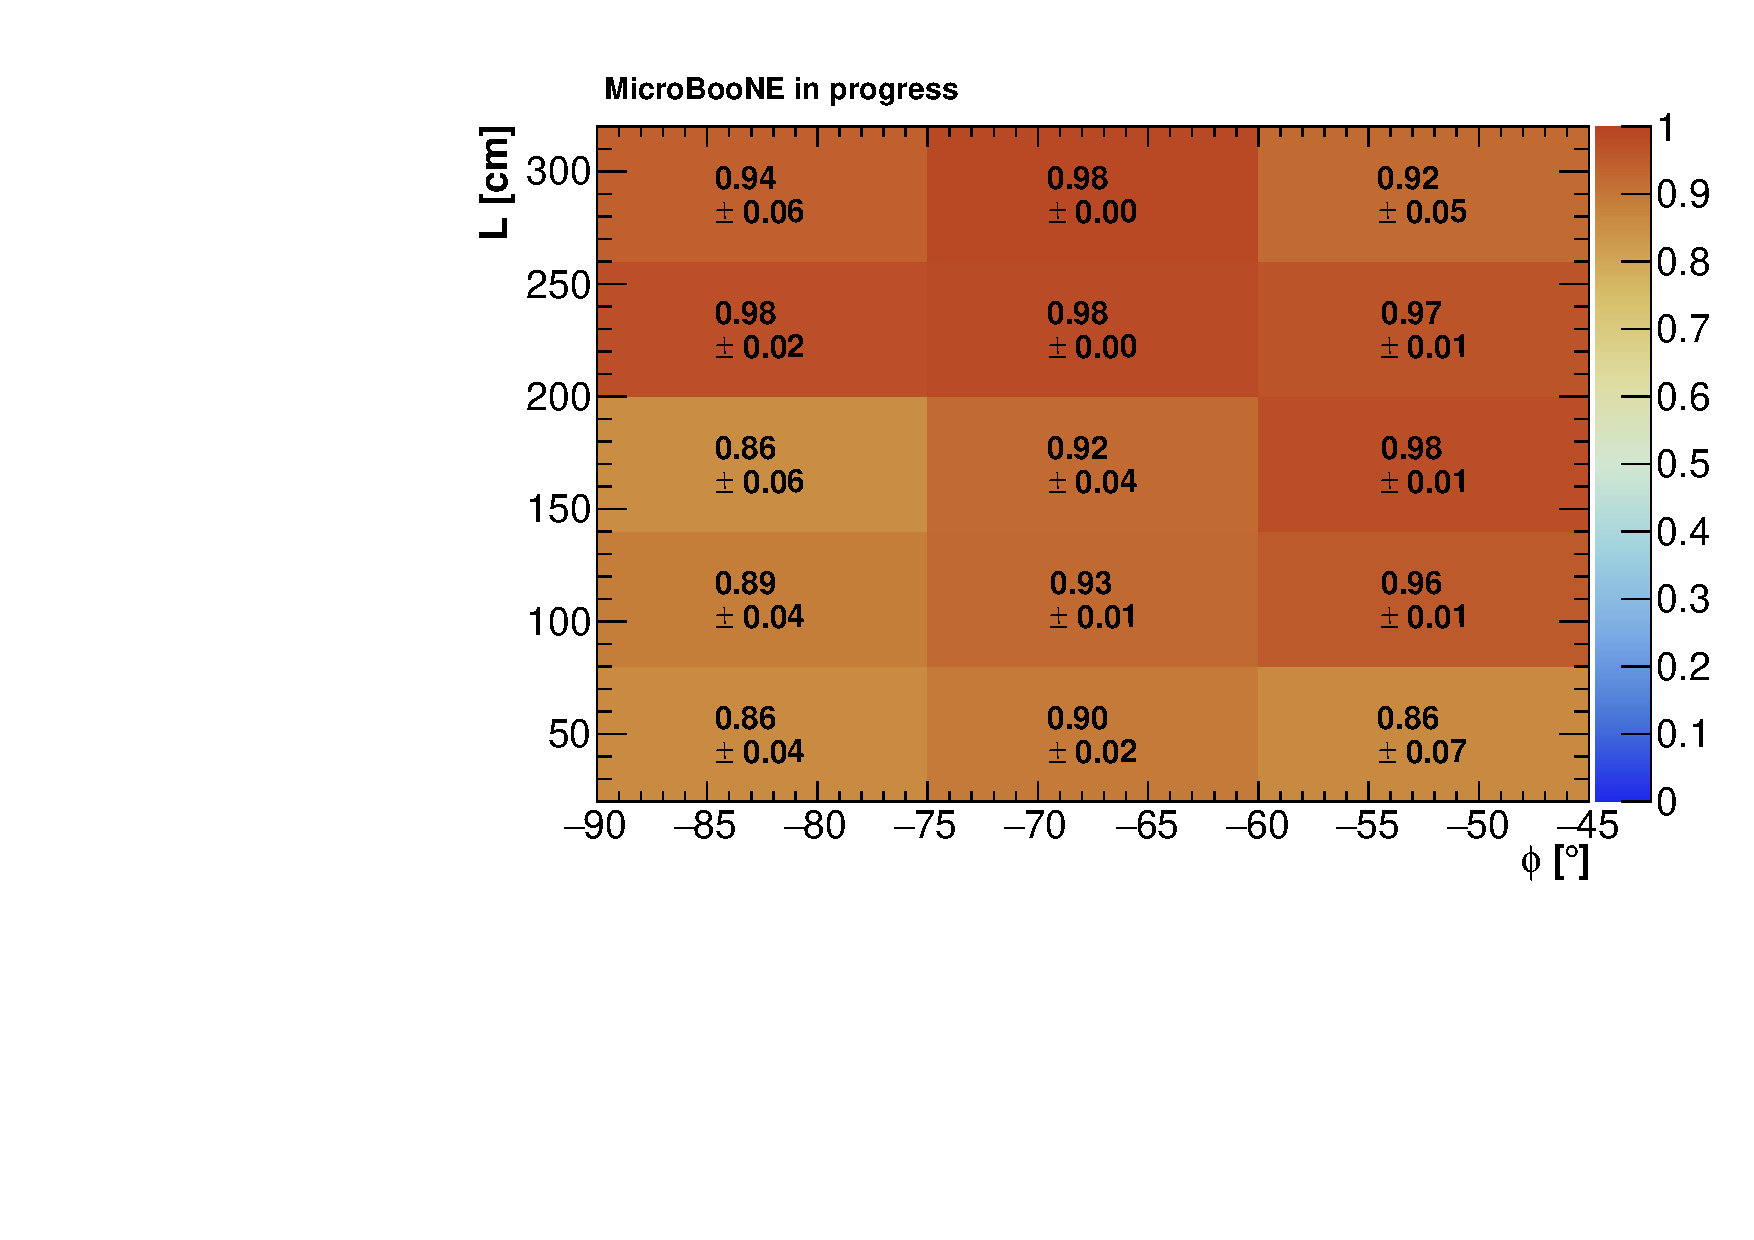
\includegraphics[width=\linewidth]{figures/e_phi_l.pdf}
  \caption{$(\phi,L)$ - Data}
\end{subfigure}\begin{subfigure}{0.33\textwidth}
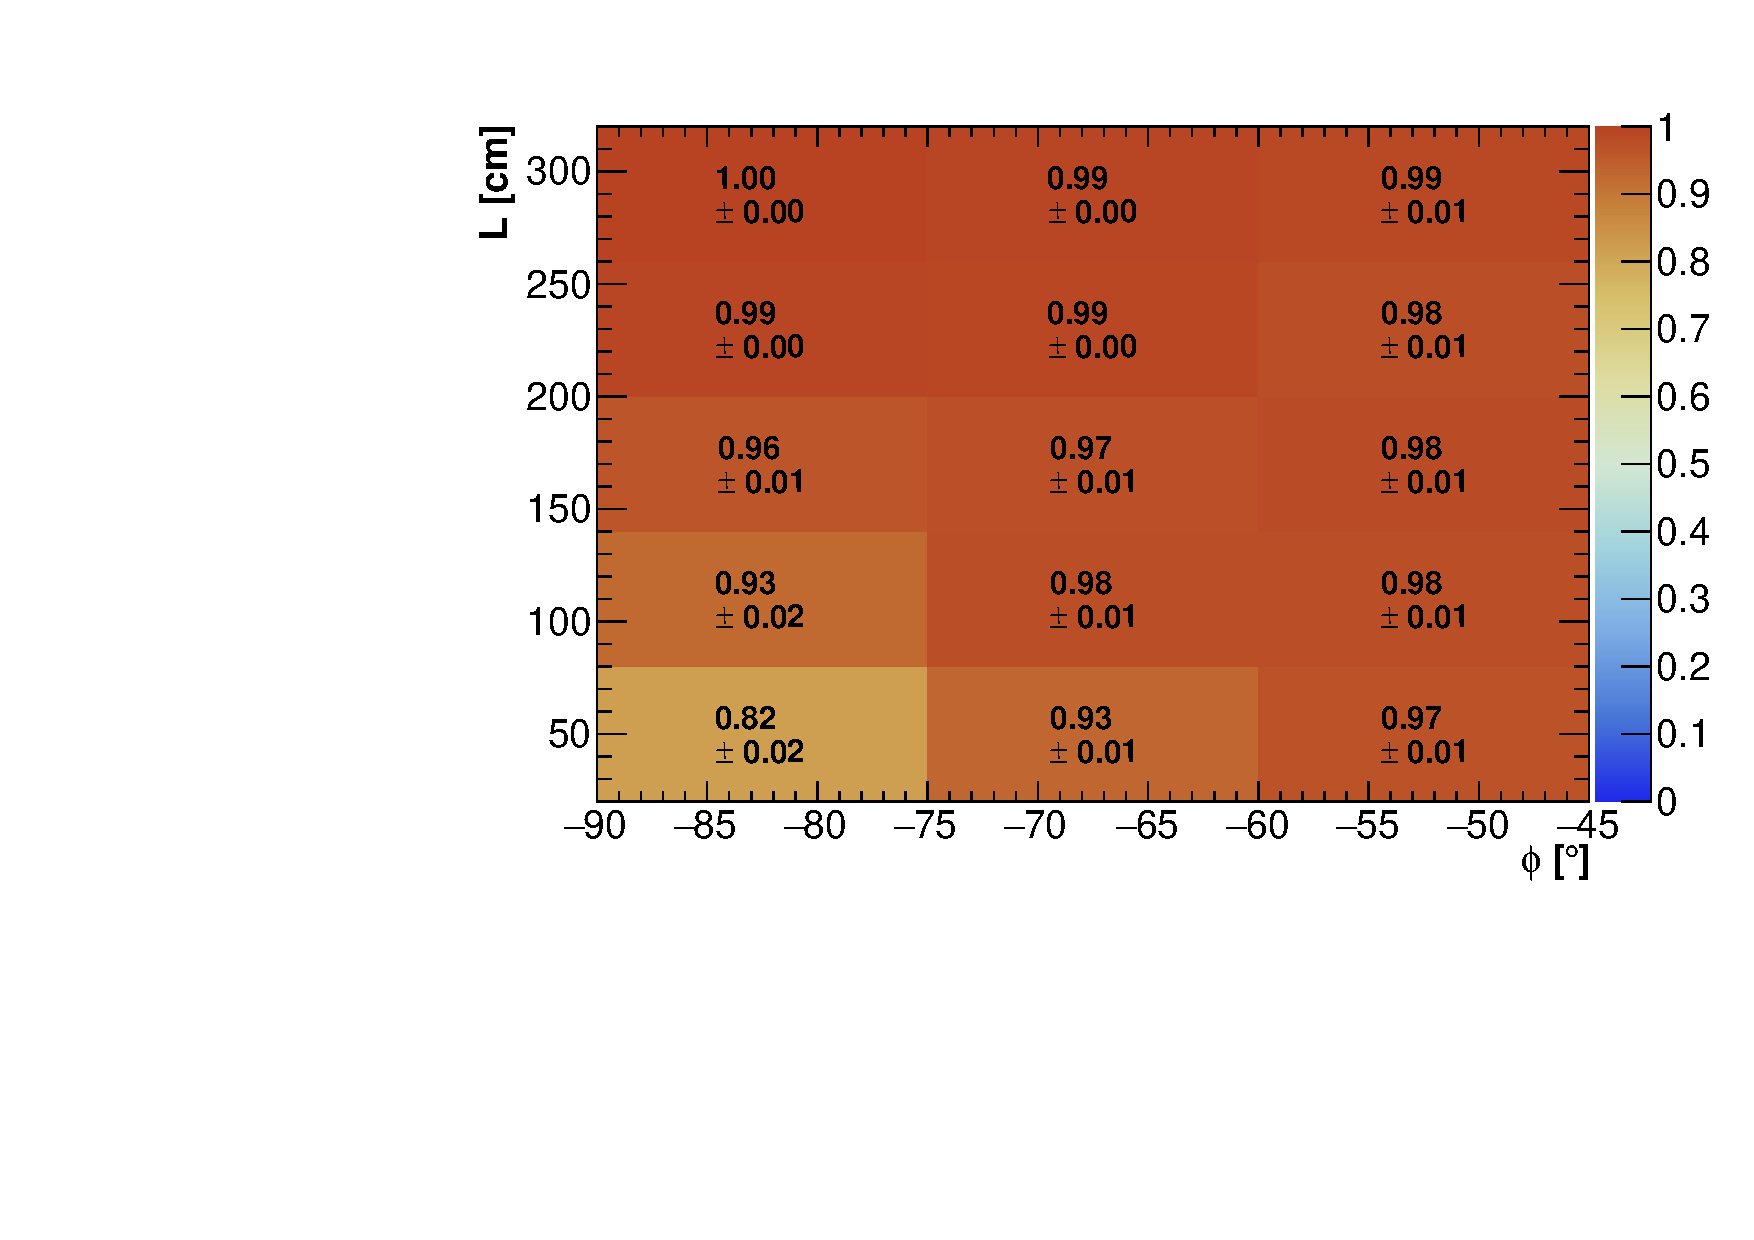
\includegraphics[width=\linewidth]{figures/phi_l_mc.pdf}
\caption{$(\phi,L)$ - Monte Carlo}
\end{subfigure}\begin{subfigure}{0.33\textwidth}
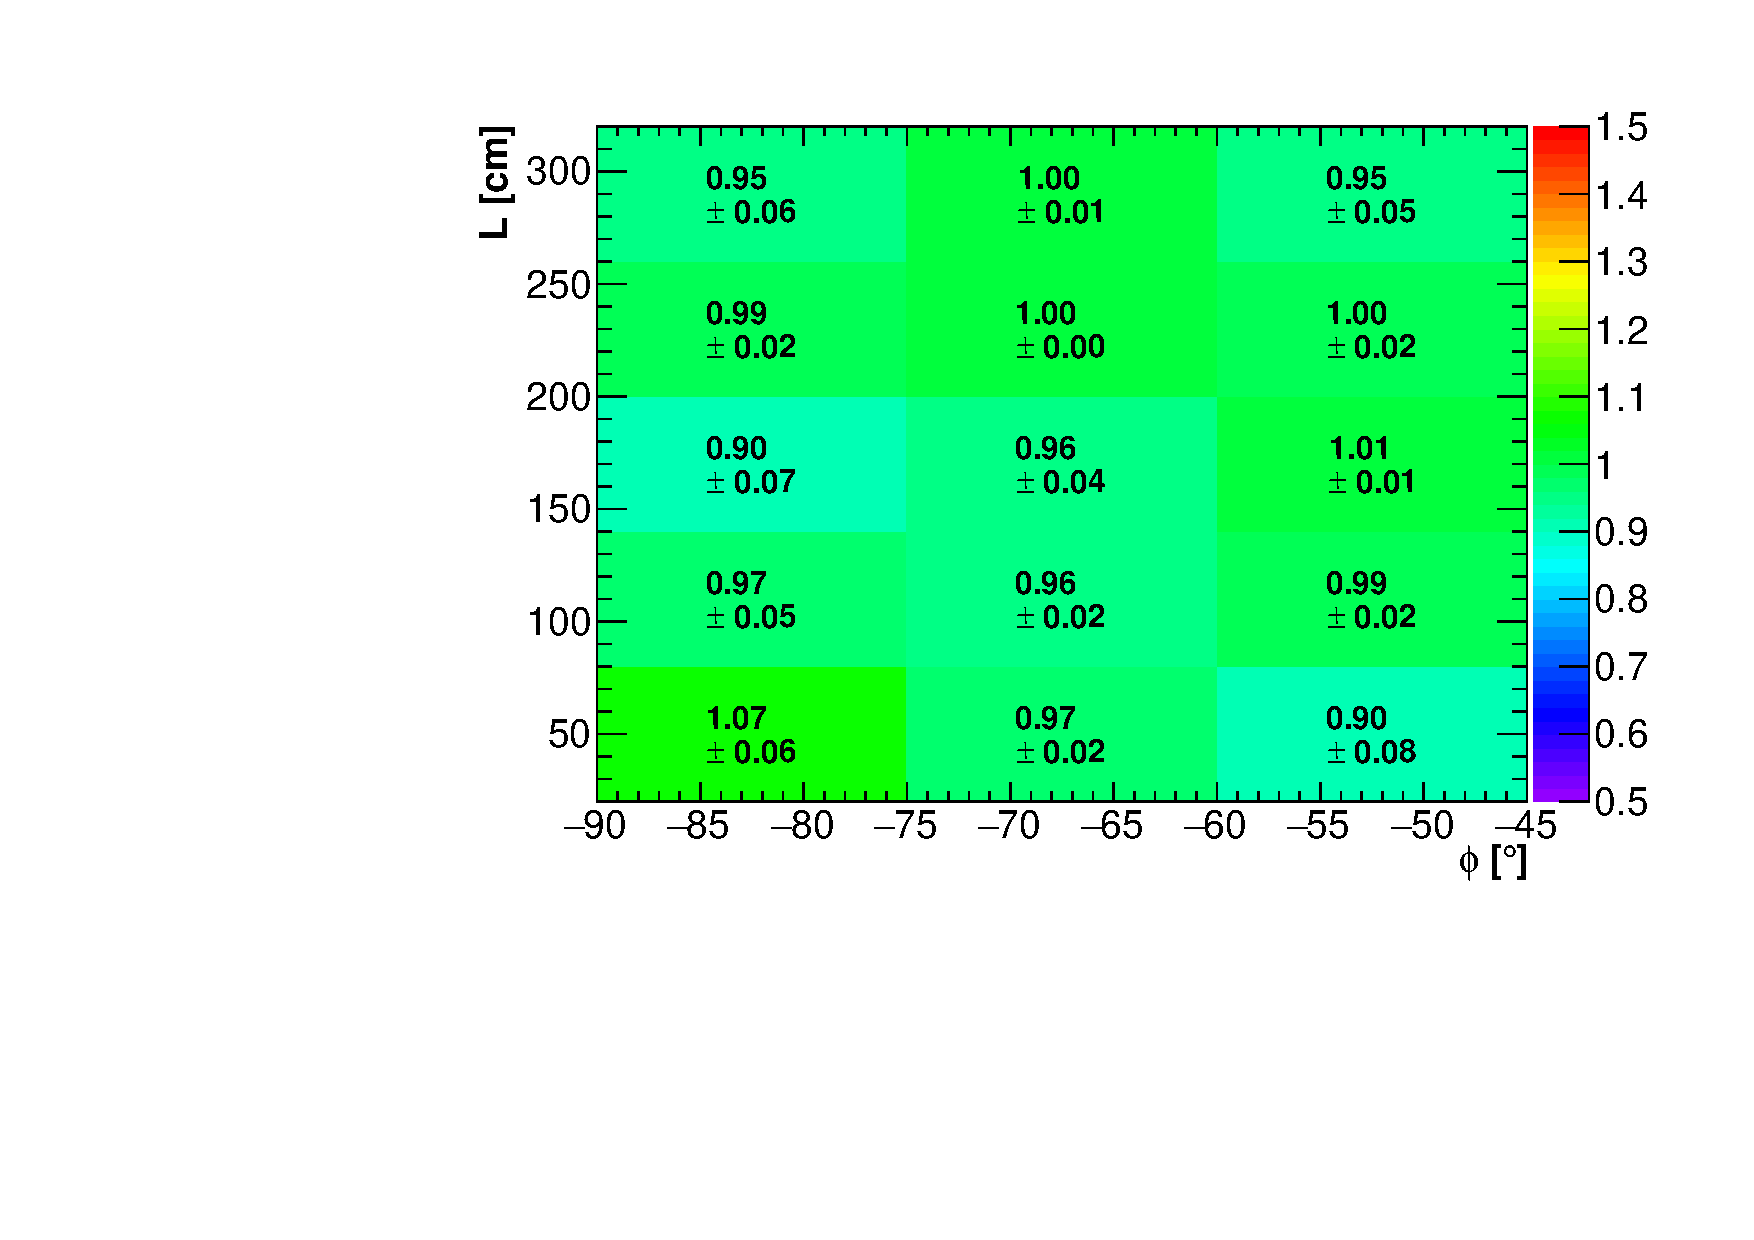
\includegraphics[width=\linewidth]{figures/phi_l.pdf}
\caption{$(\phi,L)$ - Data/Monte Carlo}
\end{subfigure}
\caption{Two-dimensional reconstruction efficiencies for data (left), Monte Carlo (center) and their ratio (right). Data errors include systematic effects. Monte Carlo errors are statistical-only.}\label{fig:2d}
\end{figure}

\begin{figure}[htbp]
  \begin{center}
    \begin{subfigure}{0.5\textwidth}
      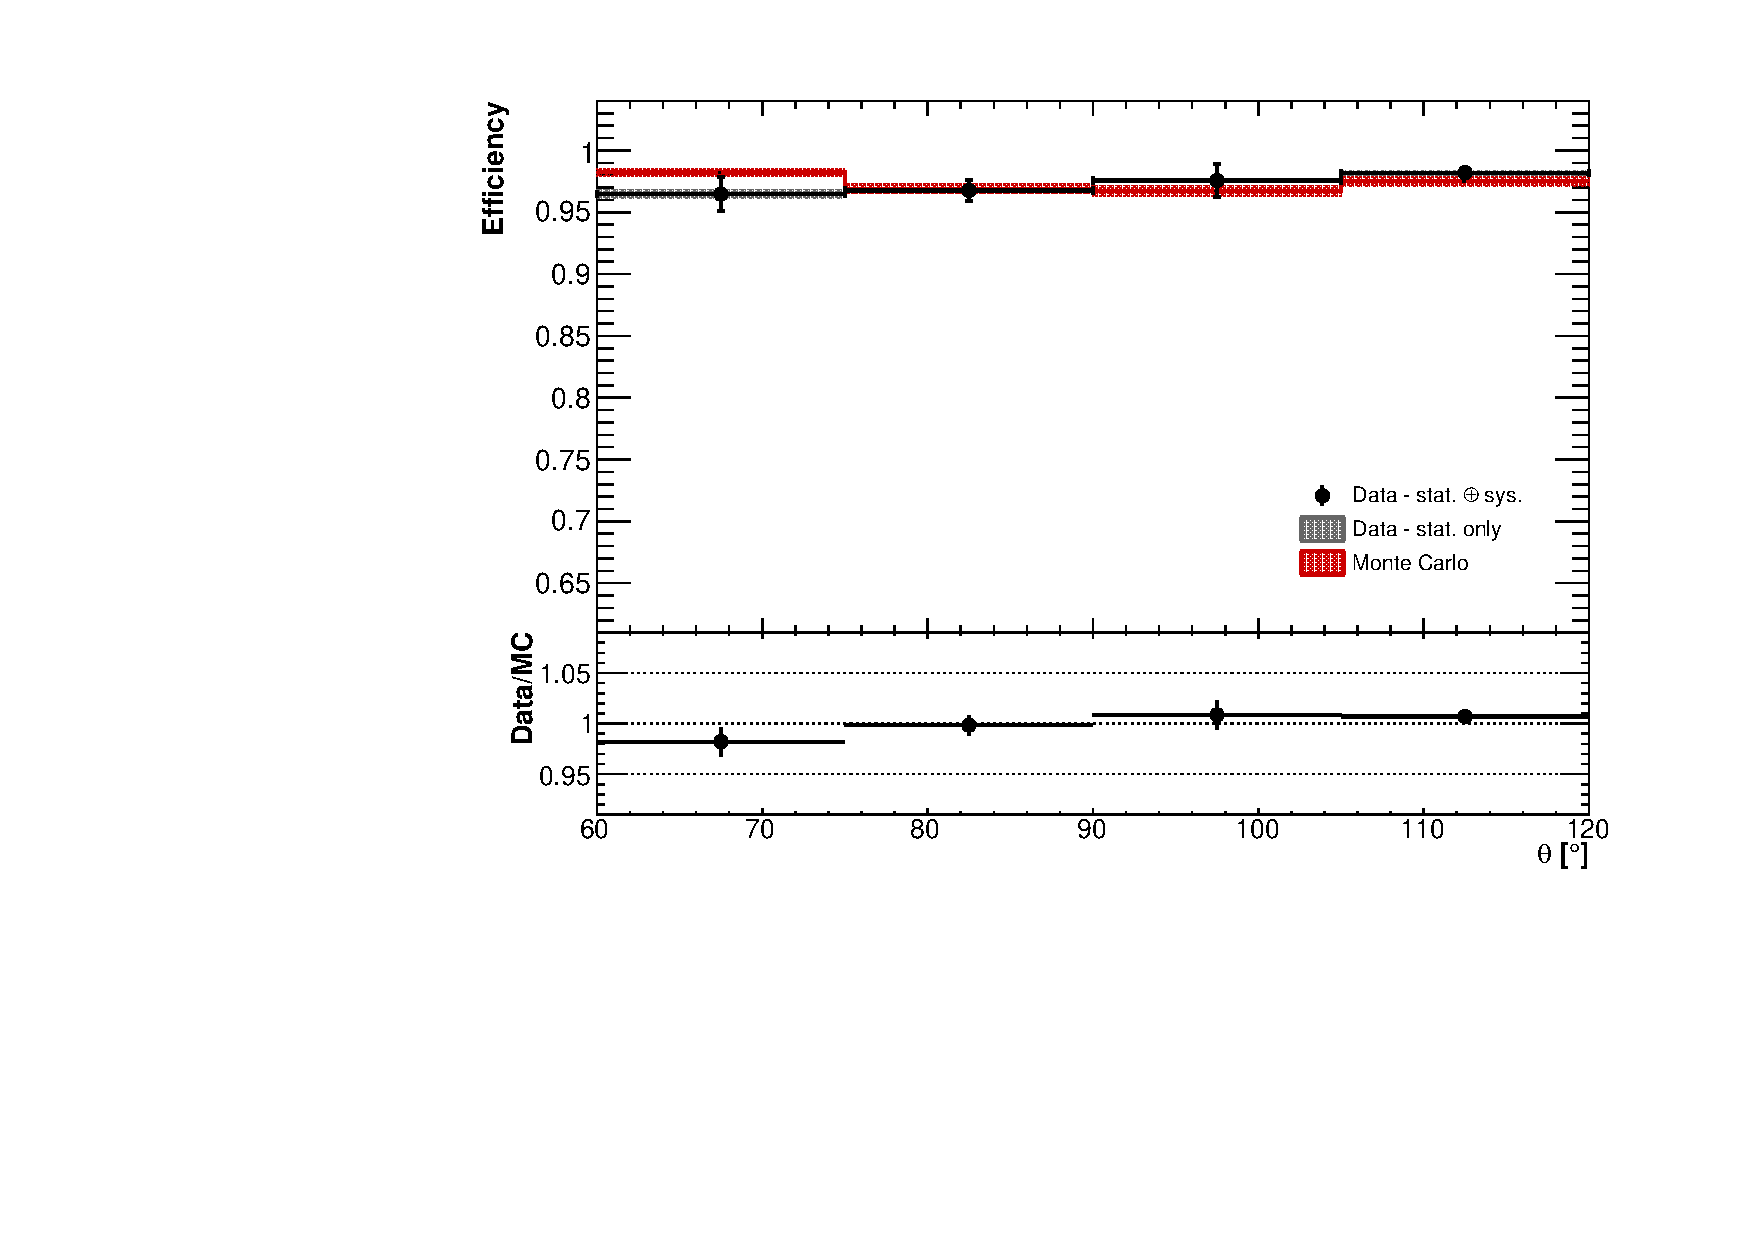
\includegraphics[width=\linewidth]{figures/theta.pdf}
      \caption{$\theta$} \label{fig:theta}
    \end{subfigure}\begin{subfigure}{0.5\textwidth}
      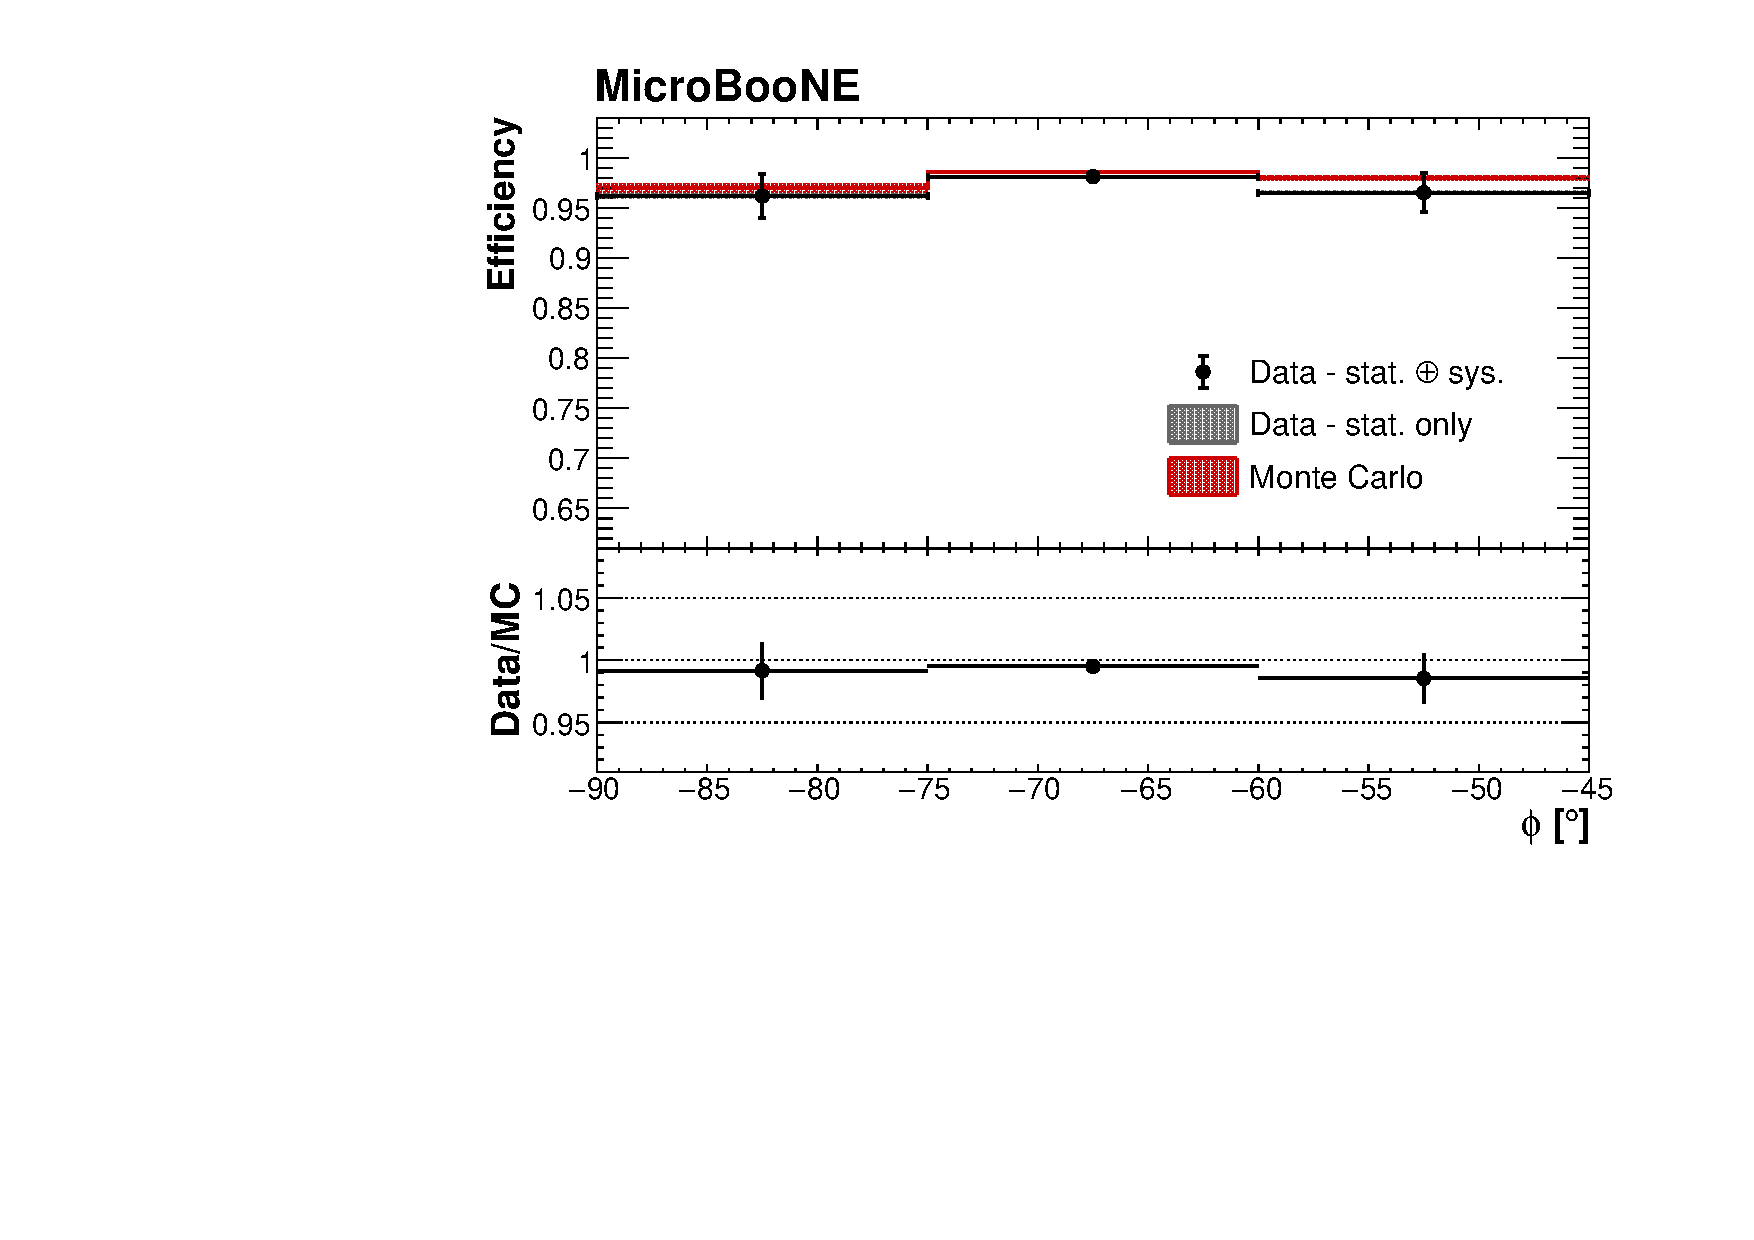
\includegraphics[width=\linewidth]{figures/phi.pdf}
      \caption{$\phi$} \label{fig:phi}
    \end{subfigure}
    \begin{subfigure}{0.5\textwidth}
      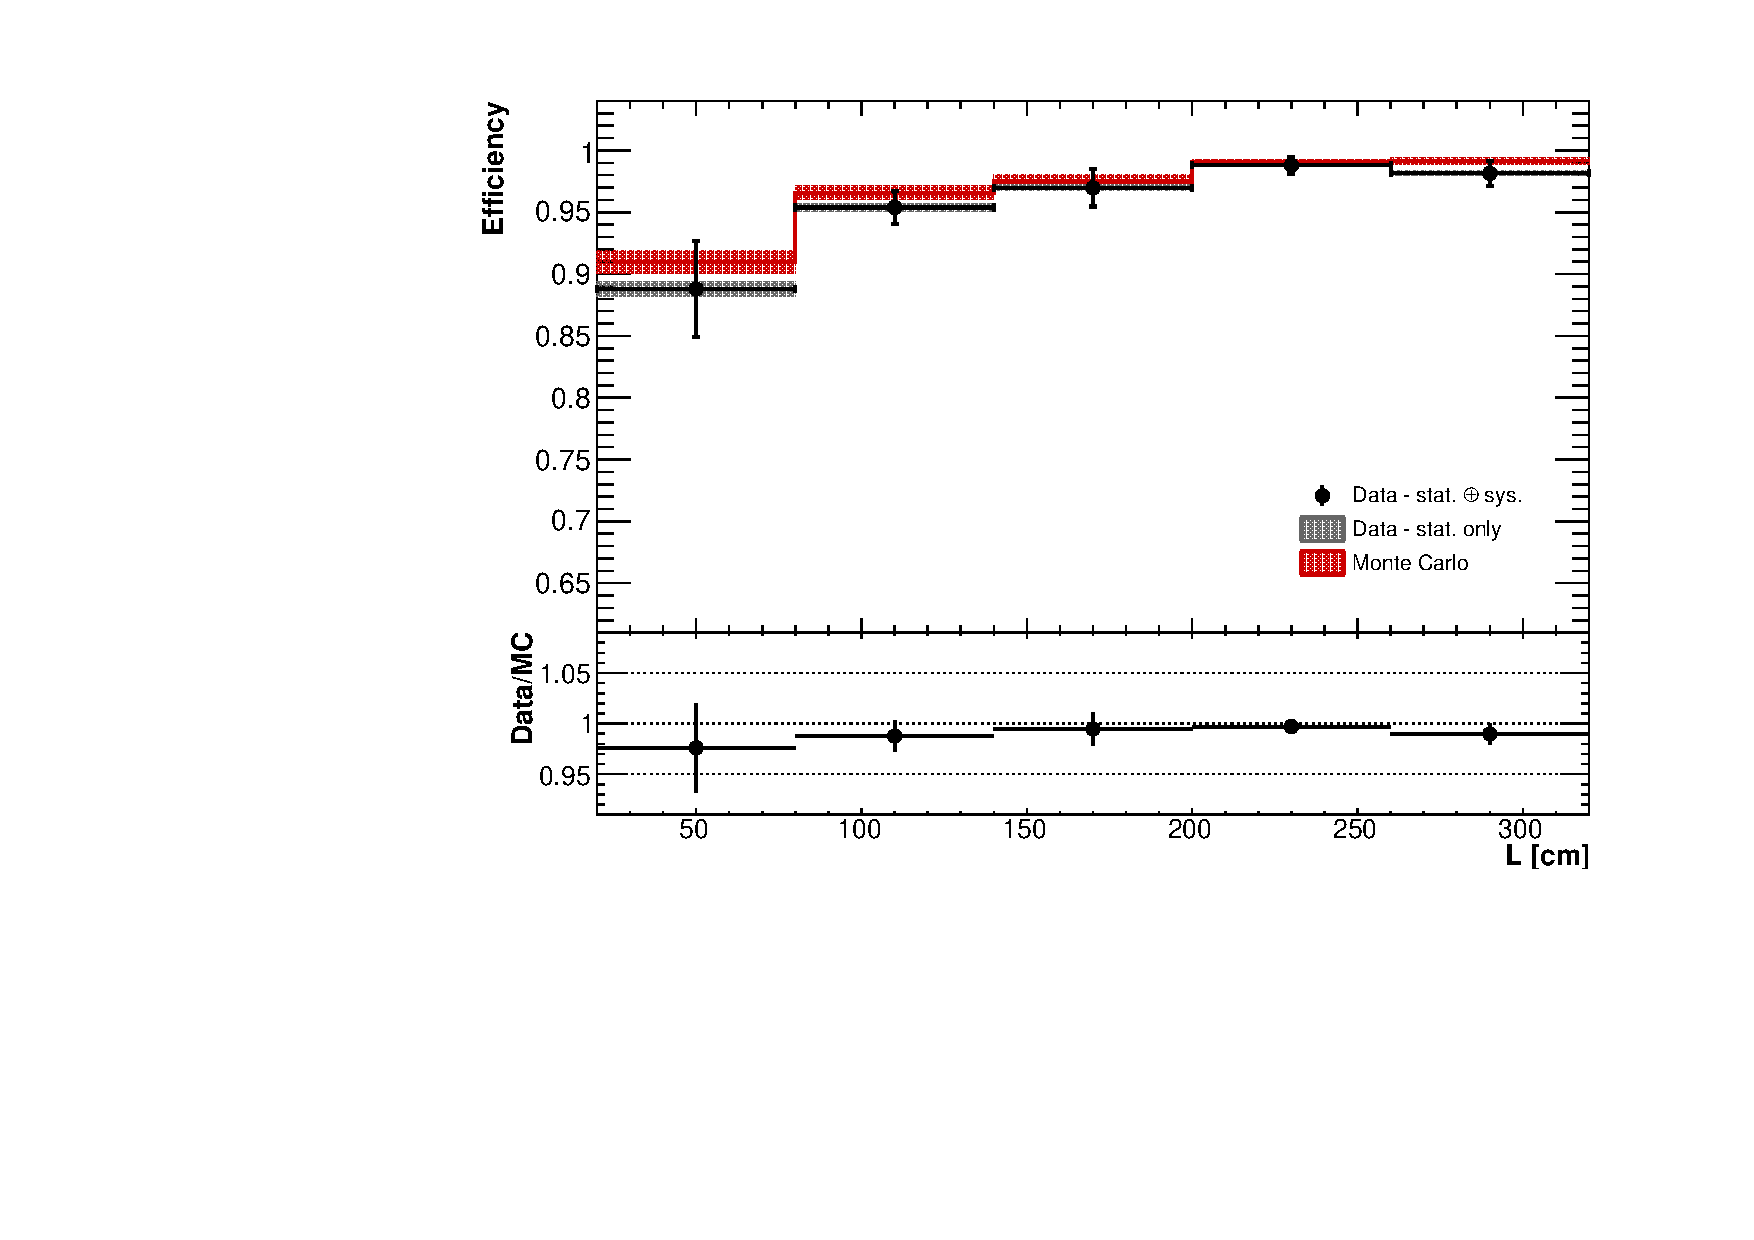
\includegraphics[width=\linewidth]{figures/l.pdf}
      \caption{$L$} \label{fig:l}
    \end{subfigure}
    \caption{Monte Carlo (red line) and data (black points) reconstruction efficiency as a function of the starting angles $\theta$, $\phi$ and the extrapolated track length $L$. Data errors include systematic effects. Monte Carlo errors are statistical-only.}\label{fig:1d}
  \end{center}
\end{figure}

As expected, the reconstruction efficiency increases with the expected track length $L$ in the TPC, since longer tracks correspond, in general, to a larger number of hit wires and they are then easier to reconstruct.

Taking into account the systematic uncertainties given by (1) the $P/A$ correcting factor (0.2\%, section \ref{sec:reco}), (2) the decay-in-flight correction factor (0.1\%, section \ref{sec:dif}), and (3) the detector non-uniformities (1.1\%, section \ref{sec:wires}), the obtained data/Monte Carlo agreement is good.%, with 46 out of 48 ($\theta,\phi,L$) bins with a data/Monte Carlo ratio within 2$\sigma$ of unity.

The overall reconstruction efficiencies, obtained integrating the three-dimensional plots and considering the systematic uncertainties, are:
\begin{align*}
\epsilon_{\mathrm{data}} &= 97.1 \pm 0.1~\mathrm{(stat)} \pm 1.4~\mathrm{(sys)}~\%\\
\epsilon_{\mathrm{MC}} &= 97.3 \pm 0.1~\%
\end{align*} for data and Monte Carlo, showing a good agreement between the two.

\section{Conclusions}
Cosmic muons hitting a LArTPC detector can be a source of backgrounds to several analysis, especially for experiments located near the surface like MicroBooNE. Measuring the reconstruction efficiency of the cosmic rays in the detector is of fundamental importance for the assessment of the detector performances and the suppression of the cosmic-ray background.

The work presented here uses the data coming from a small muon counter (the MuCS), placed on the top of MicroBooNE TPC, to measure the data reconstruction efficiency and compare it with the Monte Carlo reconstruction efficiency.
A sample of $\sim$20000 MuCS-triggering cosmic muons has been identified and the data coming from the MuCS has been merged with the data coming from the main detector. A method to evaluate the number of reconstructed MuCS cosmic rays has been studied using a dedicated Monte Carlo simulation.

The data reconstruction efficiency, measured comparing the number of MuCS-triggered events with the number of events with a reconstructed MuCS cosmic ray, has been measured as a function of the cosmic ray starting angles $\theta$, $\phi$ and the expected length in the TPC, $L$. The data reconstruction efficiency has been compared with the Monte Carlo reconstruction efficiency and the two values have been found to be compatible.

Systematic uncertainties that could affect the data reconstruction efficiency have been analyzed. The portion of muons triggering the MuCS but decaying or being captured before reaching the TPC is, according to a dedicated Monte Carlo simulation, 1.0\%. This factor has been taken into account in the measurement of the data reconstruction efficiency.
The MuCS data has been acquired with the two boxes placed in three different positions, covering different parts of the detector. The detector non-uniformities have been found to induce a non-negligible effect in the measurement of the data reconstruction efficiency. The related systematic uncertainty has been evaluated to be 1.1\%.

\begin{figure}[htbp]
  \begin{center}
    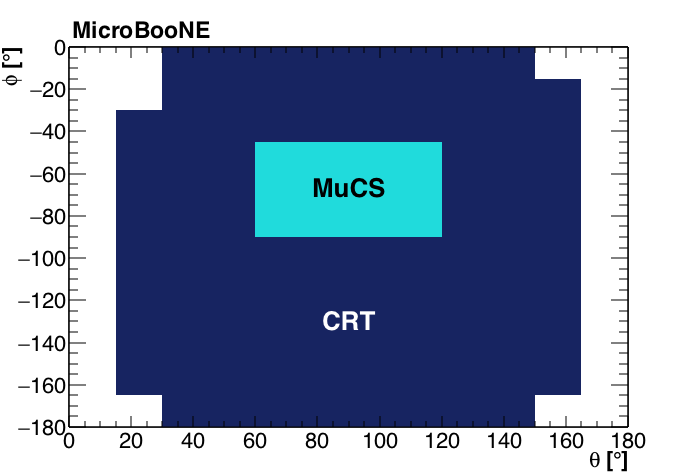
\includegraphics[width=0.7\linewidth]{figures/crt.png}
    \caption{Monte Carlo simulation of the coverage in the ($\theta,\phi$) plane for both the MuCS (light blue), as presented in this paper, and the CRT system (dark blue).} \label{fig:crt}
  \end{center}
\end{figure}

This paper validates the method of using an external muon counter to measure the cosmic-ray reconstruction efficiency in a LArTPC. The ($\theta, \phi, L$) parameter space covered by the MuCS will be expanded using the data coming from the Cosmic Ray Tagger system (CRT), installed in August 2016. This detector will be able to tag $\sim$80\% of the cosmic rays hitting the TPC and check the presence of non-uniformities in every part of the detector. The data coming from the CRT will allow to measure efficiency-corrected quantities, such as the cosmic-ray flux. Figure \ref{fig:crt} shows the coverage on the ($\theta,\phi$) plane of both the MuCS and the CRT, obtained with a Monte Carlo simulation.



\acknowledgments

This material is based upon work supported by the following: the U.S. Department of Energy, Office of Science, Offices of High Energy Physics and Nuclear Physics; the U.S. National Science Foundation; the Swiss National Science Foundation; the Science and Technology Facilities Council of the United Kingdom; and The Royal Society (United Kingdom). Fermilab is operated by Fermi Research Alliance, LLC under Contract No. DE-AC02-07CH11359 with the United States Department of Energy. The Muon Counter System and its dedicated DAQ were provided by the Virginia Polytechnic Institute and State University externally to the MicroBooNE collaboration. The Muon Counter System electronics was provided by the Nevis Laboratories of the Columbia University, under the Double Chooz project.

\clearpage{}


% We suggest to always provide author, title and journal data:
% in short all the informations that clearly identify a document.
\begin{thebibliography}{99}
  \bibitem{detector} R. Acciarri, et al. [MicroBooNE Collaboration], \textit{Design and Construction of the MicroBooNE Detector}, 2016  [\href{https://arxiv.org/abs/1612.05824}{\texttt{hep-ex/1612.05824}}].

  \bibitem{miniboone} A.~A.~Aguilar-Arevalo et al. [MiniBooNE Collaboration], \textit{Improved Search for $\bar \nu_\mu \rightarrow \bar \nu_e$ Oscillations in the MiniBooNE Experiment}, Phys.\ Rev.\ Lett.\  {\bf 110} (2013) 161801 \texttt{doi:10.1103/PhysRevLett.110.161801 [hep-ex/1303.2588]}.

  \bibitem{dune} R.~Acciarri, et al. [DUNE Collaboration], \textit{Long-Baseline Neutrino Facility (LBNF) and Deep Underground Neutrino Experiment (DUNE) : Volume 1: The LBNF and DUNE Projects}, [\href{https://arxiv.org/abs/1601.05471}{\texttt{ins-det/1601.05471}}].

  \bibitem{mcdata} R. Acciarri, et al. [MicroBooNE Collaboration], \textit{A Comparison of Monte-Carlo Simulations and Data from MicroBooNE}, 2016 [\href{http://www-microboone.fnal.gov/publications/publicnotes/index.html}{MICROBOONE-NOTE-1014-PUB}].

  \bibitem{cosmic} R. Acciarri, et al. [MicroBooNE Collaboration], \textit{Cosmic Shielding Studies at MicroBooNE}, 2016 [\href{http://www-microboone.fnal.gov/publications/publicnotes/index.html}{MICROBOONE-NOTE-1005-PUB}].

  \bibitem{crt} M. Auger, et al., \textit{A Novel Cosmic Ray Tagger System for Liquid Argon TPC Neutrino Detectors}, submitted to Instruments, \texttt{[\href{https://arxiv.org/abs/1612.04614}{ins-det/1612.04614}]}.

  \bibitem{mucs} S.R. Soleti, \textit{The Muon Counter System for the MicroBooNE experiment}, eConf C151216, \texttt{[\href{https://arxiv.org/abs/1604.07858}{ins-det/1604.07858}]}.

  \bibitem{pandora} R. Acciarri, et al. [MicroBooNE Collaboration], \textit{The Pandora multi-algorithm approach to automated pattern recognition in LAr TPC detectors}, 2016  [\href{http://www-microboone.fnal.gov/publications/publicnotes/index.html}{MICROBOONE-NOTE-1015-PUB}].

  %\bibitem{pandora} J.~S.~Marshall and M.~A.~Thomson, \textit{The Pandora Software Development Kit for Pattern Recognition}, Eur.\ Phys.\ J.\ C 75, no. 9, 439 (2015) \texttt{doi:10.1140/epjc/s10052\-015-3659-3} \texttt{[\href{https://arxiv.org/abs/1506.05348}{data-an/1506.05348}]}.

  \bibitem{pdg} C.~Patrignani, et al. [Particle Data Group Collaboration], \textit{Review of Particle Physics}, Chin.\ Phys.\ C 40 (2016) no.10,  100001 \texttt{doi:10.1088/1674-1137/40/10/100001}.

  \bibitem{corsika} D.~Heck, et al.,
  \textit{CORSIKA: A Monte Carlo code to simulate extensive air showers}, 1998,
  \texttt{FZKA-6019}.

  \bibitem{geant} S.~Agostinelli, et al. [GEANT4 Collaboration], \textit{GEANT4: A Simulation toolkit}, Nucl.\ Instrum.\ Meth.\ A {506}, 250 (2003).

  \bibitem{sce} R. Acciarri, et al. [MicroBooNE Collaboration], \textit{Space Charge Effect Measurements and Corrections}, 2016 [\href{http://www-microboone.fnal.gov/publications/publicnotes/index.html}{MICROBOONE-NOTE-1018-PUB}].

  \bibitem{besiii} W.~L.~Yuan, et al., \textit{Study of tracking efficiency and its systematic uncertainty from $J/\psi \to p \overline{p} \pi^+ \pi^-$ at BESIII}, Chin.\ Phys.\ C 40 (2016) no.2,  026201 \texttt{doi:10.1088/1674-1137/40/2/026201}  \texttt{[\href{https://arxiv.org/abs/1506.05348}{hep-ex/1507.03453}]}.


% Please avoid comments such as "For a review'', "For some examples",
% "and references therein" or move them in the text. In general,
% please leave only references in the bibliography and move all
% accessory text in footnotes.

% Also, please have only one work for each \bibitem.


\end{thebibliography}
\end{document}
